
\documentclass[a4paper, 12pt, twoside, headsepline=true]{scrartcl} % headsepline ist für die Linie unter der Kopfzeile verantwortlich

% Package für Sprachformatierung und Spellchecks
% http://ctan.space-pro.be/tex-archive/macros/latex/contrib/polyglossia/polyglossia.pdf
\usepackage{polyglossia}
\setdefaultlanguage[spelling=new]{german}

% Package zum Ändern von Headern & Footers
% mirrors.ctan.org/macros/latex/contrib/koma-script/doc/scrguien.pdf
\usepackage[automark]{scrlayer-scrpage}
\clearpairofpagestyles
\ihead{\headmark}
\ohead{\pagemark}

\pagestyle{scrheadings}
\setkomafont{pageheadfoot}{\small}

% Package zum Festlegen von Zeilenabstand
% https://www.namsu.de/Extra/pakete/Setspace.html
\usepackage[onehalfspacing]{setspace}
\setmainfont{Charis SIL} % set the main body font (\textrm), assumes Charis SIL is installed
\setlength{\parindent}{0pt}


\usepackage{csquotes}

% Package für das Referenzieren von Quellen aus .bib-Datei
\usepackage[style=ieee]{biblatex}
\addbibresource{mybib.bib}

% Package zum "Patchen" von Befehlen
% http://vesta.informatik.rwth-aachen.de/ftp/pub/mirror/ctan/macros/latex/contrib/xpatch/xpatch.pdf
% Überschreibt biblatex-Funktionalität, damit keine leeren Jahresklammern gedruckt werden
\usepackage{xpatch}
\xpatchbibdriver{online}
{\printtext[parens]{\usebibmacro{date}}}
{\iffieldundef{year}
	{}
	{\printtext[parens]{\usebibmacro{date}}}}
{}
{\typeout{There was an error patching biblatex-ieee (specifically, ieee.bbx's @online driver)}}

% Package zum Anpassen von enumerations-items 
% https://de.wikibooks.org/wiki/LaTeX-W%C3%B6rterbuch:_enumitem
\usepackage{enumitem}
\renewcommand{\labelitemiii}{$\star$}

% Package für die Anpassung der Seitengestaltung, z.B. Seitenränder
% https://www.namsu.de/Extra/pakete/Geometry.html
\usepackage{geometry}

% Package für Tabellengestaltung mit horizontalen Trennlinien
% https://www.namsu.de/Extra/pakete/Booktabs.html
\usepackage{booktabs}

% Package für Gestaltung und Anpassung einzelner Tabellenzellen 
% http://babyname.tips/mirrors/ctan/macros/latex/contrib/makecell/makecell.pdfx
\usepackage{makecell}

% Package für Positionierung von "floats", also nichtfesten Elementen wie Tabellen oder Bildern, die sich je nach Textgestaltung verschieden auf der Seite befinden müssen
% http://vesta.informatik.rwth-aachen.de/ftp/pub/mirror/ctan/macros/latex/contrib/float/float.pdf
\usepackage{float}

% Package für Tabellengestaltung 
%siehe https://www.namsu.de/Extra/pakete/Ltxtable.html
\usepackage{ltxtable}
\usepackage{filecontents}

% Package zum Anpassen von Macros/KeyValue-Daten. Hab ich garnicht verwendet, glaube ich
% http://mirrors.ibiblio.org/CTAN/macros/latex/contrib/adjustbox/adjustbox.pdf
\usepackage[export]{adjustbox}

% Package für Verwaltung von Acronymen 
% https://www.namsu.de/Extra/pakete/Acronym.html
\usepackage[printonlyused]{acronym}

% Package zum Implementieren von Textlinks
% https://www.namsu.de/Extra/pakete/Hyperref.html
\usepackage[
german,
colorlinks=true,
linkcolor=blue, % einfache interne Verknüpfungen
%TODO: Folgende Zeile für Druckdokument verwenden!
%hidelinks=true
anchorcolor=black,% Ankertext
citecolor=green, % Verweise auf Literaturverzeichniseinträge im Text
urlcolor=cyan % Farbe der URLs
%Back-Links zu den Kapiteln
]{hyperref}
\apptocmd{\UrlBreaks}{\do\f\do\m}{}{}
\setcounter{biburllcpenalty}{9000}% Kleinbuchstaben
\setcounter{biburlucpenalty}{9000}% Großbuchstaben
\setcounter{biburlnumpenalty}{9000}% Zahlen
%\usepackage[german,draft]{hyperref}

%Neudefinition für den Name von Subsubsection, damit "Unterunterabschnitt" nicht bei Referenzen auftaucht
\def\subsubsectionname{Unterabschnitt}%
\def\subsubsectionautorefname{Unterabschnitt}%

% Package für besseren Umgang mit Grafiken
% http://ftp.gwdg.de/pub/ctan/macros/latex/required/graphics/grfguide.pdf
\usepackage{graphicx}

% Package für Platzieren von Bildern neben/im Text
% https://www.namsu.de/Extra/pakete/Wrapfig.html
\usepackage{wrapfig}
\newcommand{\myhline}{\noalign{\global\arrayrulewidth0,1cm}\hline
	\noalign{\global\arrayrulewidth1pt}}
% Umbenennung der Caption Beschreibung unter Bildern von "Abbildung" in "Abb." um Platz zu sparen.
\addto\captionsgerman{%
	\renewcommand{\figurename}{Abb.}%
}

% Definiere eine neue Liste bei der die Unterpunkte auch nummeriert sind, wie bei einem Inhaltsverzeichnis.
\newlist{legal}{enumerate}{10}
\setlist[legal]{label*=\arabic*.}
%\setcounter{tocdepth}{4}
%\setcounter{secnumdepth}{4}

\makeatletter 
\@addtoreset{figure}{section} 
\@addtoreset{table}{section} 
\makeatother 

%Commands zum Neustarten der Seitennummerierung ab Inahltsverzeichnis, falls vorher noch Titelseiten o.Ä. folgen
\renewcommand{\thefigure}{\thesection.\arabic{figure}} 
\renewcommand{\thetable}{\thesection.\arabic{table}} 

\begin{document}
% Nötig um in der PDF Datei einen Lesezeicheneintrag für das Inhaltsverzeichnis zu bekommen.
\pdfbookmark[1]{Inhaltsverzeichnis}{toc}
\tableofcontents
\clearpage
\newpage

\addsec{Abkürzungsverzeichnis}

\pdfbookmark[2]{Abkürzungsverzeichnis}{toc}
% Angabe in eckigen Klammern sollte das längste Acronym enthalten.
% Das ist notwendig damit sich der Einschub am längsten Acronym orientiert.
\begin{acronym}[header=Abkürzungsverzeichnis]
	\acro{arm}[ARM]{Architectural Reference Model}
	\acro{bpd}[BPD]{Business Process Diagram}
	\acro{bpel}[BPEL]{Business Process Execution Language}
	\acro{bpm}[BPM]{Business Process Management}
	\acro{bpmn}[BPMN]{Business Process Model and Notation}
	\acro{bpmn4cps}[BPMN4CPS]{Business Process Model and Notation for Cyber-Physical Systems}
	\acro{bpms}[BPMS]{Business Process Management System/Suite}
	\acro{cmmn}[CMMN]{Case Management Model and Notation}
	\acro{cps}[CPS]{Cyber-Physical Systems}
	\acro{eoi}[EoI]{Entity of Interest}
	\acro{eepk}[eEPK]{erweiterte Ereignisgesteuerte Prozesskette}
	\acro{iapmc}[IAPMC]{IoT-aware Process Modelling Concept}
	\acro{ibpms}[iBPMS]{intelligent Business Process Management System/Suite}
	\acro{iot}[IoT]{Internet of Things}
	\acro{iota}[IoT-A]{Internet of Things - Architecture}
	\acro{m2m}[M2M]{Machine-to-Machine}
	\acro{omg}[OMG]{Object Management Group}
	\acro{p2m}[P2M]{Person-to-Machine}
	\acro{rfid}[RFID]{Radio-frequency Identification}
	\acro{uml}[UML]{Unified Modelling Language}
\end{acronym}

\clearpage

\addcontentsline{toc}{section}{Tabellenverzeichnis}

\listoftables

\clearpage

\addcontentsline{toc}{section}{Abbildungsverzeichnis}
\listoffigures
\clearpage


\section{Einleitung} \label{sec:section}
%TODO Kurzer Absatz, Ziel dieser Thesis ist ...
%TODO Einleitung muss am Ende besser an den Inhalt angepasst werden
Ziel dieser Thesis ist die Konzeption eines Modellierungsansatzes für \ac{iot}
Workflows. Hierfür werden grundlegende Besonderheiten von \ac{iot} Workflows festgehalten und davon ausgehend Evaluierungskriterien für die Bewertung gängiger Modellierungsansätze abgeleitet. Anhand der Kriterien werden Modellierungsmethoden bewertet und mögliche Erweiterungsmöglichkeiten vorgestellt. Der daraus resultierende Ansatz wird auf vorhandene Use-Cases angewandt und bewertet.

\subsection{Motivation} \label{sec:subsection}
Das \ac{iot} ist eines der größten IT-Buzzwords der letzten Jahre und beschreibt die durch eingebettete Elektronik ermöglichte Vernetzung von physischen Dingen. Die dadurch gewonnen Daten bzw. Ereignisse, bieten neben dem Potential der Prozessoptimierung und Erweiterung die Möglichkeit zur Generierung völlig neuer Geschäftsprozesse und Modelle. 
Das Weiteren sinken die Kosten physische Dinge mit Sensoren auszustatten und untereinander zu vernetzen, was zu einer hohen Anzahlvon \ac{iot} Projekten führt. Laut Gartner sollen im Jahr 2020 mehr als die Hälfte der wichtigsten Geschäftsprozess Elemente des \ac{iot} beinhalten \cite{garnteriotgrowth}. Da der Wettbewerb auf dem Technologiemarkt rasant zu nimmt, ist es unerlässlich sich von der Konkurrenz abzuheben. Die Verwaltung von IoT Geräten, sogenannten Smart Devices, mit \ac{bpm} ermöglicht eine einfache Wartung ihrer Orchestrierung. Des weiteren bietet es die Möglichkeit der Nachverfolgung, die es erlaubt KPIs über die Prozesse und Devices einfach zu ermitteln. Diese KPIs sind maßgebend für ein effektives Arbeiten mit der stetig wachsenden Anzahl von Devices \cite{bpmofthings}.

\subsection{Problemstellung} 
Während sich das IoT im Allgemeinen auf Kommunikation und Datenfluss konzentriert, berücksichtigen \ac{bpm}-Ansätze den Kontrollfluss, große monolithische Prozessmodelle und asynchrone Interaktionen. Darüber hinaus haben die meisten BPM-Ansätze Probleme mit nicht routinemäßigen, nicht deterministischen Prozessen, während IoT-Anwendungen typischerweise solche Interaktionen beinhalten. Das Problem der Vereinigung von \ac{iot} und \ac{bpm} beginnt bereits bei der Darstellung und Modellierung der neuen Geschäftsprozesse, da Standards wie \ac{bpmn} nur bedingt hierfür geeignete Elemente vorsehen. Das aufkommen der überwältigenden Datenmenge sorgt dafür, dass Objekte selbständige Routinen, sogenannte Verhaltensmuster oder Gewohnheiten ausführen. Dieses selbständige Handeln ohne zentrale Steuerung macht die Modellierung umfassender End-to-End Prozesse praktisch unmöglich. Dementsprechend müssen diese Verhaltensmuster als sogenannte event-driven micro processes organisiert werden. Da die Wechselwirkungen zwischen diesen Mikroprozessmodellen nicht auf der niedrigen Ebene des Nachrichtenaustausches beschrieben werden können, müssen diese laut "The Internet-of-Things Meets Business Process Management: Mutual Benefits and Challenges" auf einer höheren semantischen Ebene beschrieben werden \cite{iotmeetsbpm}. Diese Problemstellungen bilden die Grundlage für diese Thesis.
%TODO Quelle zu event driven Microprocesses eventuell mit Bild 
%event driven microprocesses erklären

\subsection{Aufbau der Thesis}
Nach der Einleitung mit Motivation, Problemstellung, Zielsetzung sowie dem Aufbau der Thesis folgen Grundlagen im Bereich des \ac{iot}, der Prozess Modellierung sowie des \ac{bpm}, welche zum Verständnis der weiteren Arbeit dienen.
 
 Im Hauptteil werden typische Muster von \ac{iot} Workflows identifiziert. Aus den Mustern werden Unterschiede und Besonderheiten zwischen \ac{iot} Workflows und Workflows ohne \ac{iot} Integration herausgearbeitet, welche bei der Modellierung zu berücksichtigen sind. Folgend werden die bestehenden Modellierungskonzepte \ac{iota} und \ac{bpmn4cps} vorgestellt.
 Anhand der Unterschiede werden Evaluierungskriterien für die Geschäftsprozess Modellierung abgeleitet. Diese Evaluierungskriterien werden im Anschluss dazu verwendet um bestehende Modellierungsmethoden auf ihre Eignung zur Modellierung von \ac{iot} Workflows zu bewerten. Basierend auf der Bewertung wird ein Modellierungskonzept für \ac{iot} Workflows erarbeitet. Zur Evaluierung werden mehrere Use-Cases analysisiert und das entwickelte Modellierungskonzept darauf angewandt. Anhand der Ergebnisse wird das Modellierungskonzept bewertet.
 
Im Schlussteil wird das Ergebnis festgehalten, ein Fazit getroffen und weiterführende Arbeiten sowie ein Ausblick vorgestellt.
 
\newpage

\section{Grundlagen} \label{sec:section2}
In diesem Kapitel werden zunächst Grundlagen des \ac{iot} erläutert. Anschließend werden die wichtigsten Modellierungsmethoden für Prozesse dargestellt und Grundlagen des \ac{bpm} erklärt. Zum Abschluss werden zwei Erweiterungen von \ac{bpmn} zur Modellierung von \ac{iot} Workflows vorgestellt.

\subsection{BPM}
Laut der Defintion von bpm.com, der größten Internetseite im Bezug auf Artikel, Nachrichten, Forschung und Veröfftentlichungen für \ac{bpm} \cite{aboutbpmcom} versteht sich \ac{bpm} als: "eine Disziplin, die eine beliebige Kombination aus Modellierung, Automatisierung, Ausführung, Kontrolle, Messung und Optimierung von Geschäftsabläufen zur Unterstützung von Unternehmenszielen, übergreifenden Systemen, Mitarbeitern, Kunden und Partnern innerhalb und außerhalb der Unternehmensgrenzen umfasst"\cite{whatisbpm}. \ac{bpm}, in seinem Kern, nutzt den Workflow, um große Daten- und Informationsmengen zu verwalten, zu aktualisieren und zu verfolgen \cite{bpmofthings}. \\
Besonders von einander zu Unterscheiden sind die Begriffe \ac{bpm} und \ac{bpms}. \ac{bpm} ist eine Praktik und kein Produkt. \ac{bpms} sind Produkte zum Beispiel von IBM oder Camunda. Was in den Produkten angeboten wird, hängt immer von Verkäufer des Produktes ab. \ac{bpms} sind dafür entworfen um \ac{bpm} zu unterstützen aber bieten darüber hinaus Funktionaltiäten welche nichts mit \ac{bpm} an sich zu tun haben.  
%TODO Togaf bezug einbauen.
Was genau die Kernfunktionalitäten eines \ac{bpms} sind wird im nächsten Unterkapitel beschrieben.
%TODO Quelle http://pubs.opengroup.org/architecture/togaf9-doc/arch/
%TODO BPM Lifecycle -> erster schritt process definieren 2 Schritt modellieren, Thesis augenmerk auf schritt 2
\subsubsection{BPMS}
Wie zuvor beschrieben sind \ac{bpms} dafür entworfen um die \ac{bpm} zu unterstützen. Folglich können alle Informationssysteme, die sich mit der Definition, Verwaltung, Anpassung und Bewertung von Aufgaben befassen, welche sich aus Geschäftsprozessen und Organisationsstrukturen ergeben als \ac{bpms} bezeichnen. Diese Produkte sind in der Lage, den Workflow in einer Organisation zu definieren, zu steuern, Daten zu übertragen und alte Informationssysteme, bestehende Programme und Programmmodule zu integrieren \cite{bpms}. Das Gebiet der \ac{bpms} besitzt 2017 einen geschätzten Marktwert von 14,5 Milliarden USD und lässt sich auf die grossen Anteilshaber wie IBM, Pegasystems und RedHat zurückführen \cite{bpmsmarket}.

\subsubsection{iBPMS}

Der Begriff \ac{ibpms}  wurde von Gartner geprägt und kann als natürliche Weiterentwicklung der \ac{bpms} verstanden werden. \ac{ibpms} bieten durch zusätzliche Funktionen wie zum Beispiel die Integration mit Social Media, mobile Prozessaufgaben, Streaming-Analysen sowie Echtzeit-Entscheidungsmanagement mehr "Intelligenz" in Geschäftsprozessen \cite{onibpms}.  In Tabelle \ref{table:GartnerIBPMS} werden die Kernfunktionalitäten von \ac{ibpms} und deren Erklärung dargestellt. Der Begriff \ac{ibpms} wurde von  \ac{bpms} Herstellern wie Pegasystems und Appian angenommen und in ihr Portfolio übernommen \cite{appianibpms} \cite{pegaibpms}.

\begin{filecontents}{\jobname-iBPMSTable.tex}
	\begin{longtable}{p{4.5cm}X}
		\caption{Kernfunktionalitäten eines iBPMS \cite{ibpms}}\\
		\label{table:GartnerIBPMS}
		% Definition des ersten Tabellenkopfes auf der ersten Seite
		\textbf{Funktionalität} & \textbf{Erklärung}  \\
		\hline
		\endfirsthead % Erster Kopf zu Ende
		%  Definition des Tabellenkopfes auf den folgenden Seiten
		\textbf{Funktionalität} & \textbf{Erklärung}  \\
		\hline
		\endhead % Zweiter Kopf ist zu Ende
		siehe n{\"a}chste Seite\\
		\endfoot
		\hline
		Tabelle zu Ende \\
		\endlastfoot
		% Ab hier kommt der Inhalt der Tabelle
		Interaktionsmanagement & Die Funktionalität, verschiedene Arten von Aktivitäten und Interaktionen zur Laufzeit zu orchestrieren, um die Arbeit zu unterstützen, welche von Menschen, Systemen und Dingen (wie im \ac{iot}) geleistet wird, um spezifische Geschäftsergebnisse zu erzielen.
		\\ \hline
		Hochproduktive App Generierung & Ermöglicht IT-Entwicklern, schnell und einfach eine prozessorientierte Anwendung zu erstellen.
		Anwendungen, die auf der Plattform basieren, verwenden ein Metadatenmodell, um den gesamten Lebenszyklus von Geschäftsprozessen zu verwalten und prozessbezogene Daten zu bearbeiten.
		\\ \hline
		Überwachung und Geschäftsanpassung & iBPMS Plattformen unterstützen Business Activity Monitoring um den Status von Prozessinstanzen, Fällen und anderen Verhaltensweisen in nahezu Echtzeit kontinuierlich zu überwachen.
		\\ \hline
		Regeln und Entscheidungs Management &  Softwaresysteme wie inference engines, recommendation engines und decision management capabilities, die als Orientierungshilfe dienen, um menschliche oder automatisierte betriebliche Entscheidungen nach Geschäftsrichtlinien zu treffen. %TODO Softwaresysteme erklären
		\\ \hline
		Analysen & \ac{ibpms} wenden müssen Logik und Statistiken auf Daten anwenden, um Erkenntnisse für bessere Entscheidungen zu gewinnen. Ein \ac{ibpms} kann prädiktive Analysen wie z.B. Scoring Services oder präskriptive Analysen wie z.B. optimization engines enthalten oder mit diesen in Verbindung stehen.
		\\ \hline
		Kompatibilität &  Kompatibilität mit externen Anwendungsdiensten und Systemen muss gewährleistet sein. Zu diesen Diensten und Systemen gehören benutzerdefinierte und kommerzielle Standardanwendungen sowie Cloud-basierte SaaS-Anwendungen und deren Datenbanken.
		\\ \hline
		Mobile Verwendbarkeit & Die Möglichkeit, von einer Vielzahl mobiler Geräte, einschließlich Smartphones und Tablets, auf Anwendungen zuzugreifen. Die Plattform bietet nicht nur Zugriff von jedem Ort aus, sondern optimiert auch die nativen Fähigkeiten des Mobilgeräts, einschließlich der Kamera und anderer Sensoren.
		\\ \hline
		Kontext- und Verhaltensstatistik & Die Fähigkeit der Plattform verkürzt die Zeit, welche benötigt wird, um Verhaltensweisen die zur Verbesserung der Geschäftsergebnisse erforderlich sind zu erkennen und zu optimieren. Dies kann die Analyse der vergangenen Ausführungshistorie oder die Simulation von Verhaltensvorschlägen beinhalten.
		\\ \hline
	\end{longtable}
\end{filecontents}
\LTXtable{\textwidth}{\jobname-iBPMSTable.tex}

Auch wenn \ac{ibpms} Interaction Management als eines seiner Kernfunktionalitäten besitzen muss, ist hier kein Standard für die Modellierung von \ac{iot} Workflows gegeben beziehungsweise vorgegeben. Es bleibt jedem Hersteller selbst überlassen wie die Worfklows zu modellieren sind.

\subsection{Internet of Things}

Die Idee eines Internets der Dinge hat seine Ursprünge in den Konzepten des Anfang der 90er Jahre von Mark Weiser skizzierten "Ubiquitous Computing". Dies bezeichnet er als nahtlose Einbindung von Computern in die reale Welt bezeichnet \cite{ucweiser}. \\
Grundgedanke des "Ubiquitous Computing" ist eine Erweiterung beliebiger physischer Gegenstände über ihre bestehende Form und Funktion hinaus durch mikroelektronische Komponenten \cite{237456}. Die so entstehenden "smarten" Gegenstände bilden, mit digitaler Logik, Sensorik und der Möglichkeit zur Vernetzung ausgestattet, ein Internet der Dinge.\\
 Der Begriff \acl{iot} wurde jedoch erst 1999 von Kevin Ashton im Zusammenhang eines globalen Netzwerks aus Objekten welche mit RFID angereicht wurden bei einer Präsentation bei Procter \& Gamble erstmals verwendet \cite{rfidiot}. \\
 Eine einheitliche Definition des \ac{iot} gibt es nicht, diese Thesis beruht auf der 2012 publizierten Definition aus "Overview of the IoT" der International Telecommunication Union. Diese definiert \ac{iot} als :"Eine globale Infrastruktur für die Informationsgesellschaft, die fortschrittliche Dienste ermöglicht, indem sie (physische und virtuelle) Dinge miteinander verbindet, die auf bestehenden und sich entwickelnden interoperablen Informations- und Kommunikationstechnologien basieren" \cite{iotdefinition}. \\
Aus technischer Sicht steht hinter dem Internet der Dinge weniger eine einzelne Technologie oder eine spezifische Funktionalität als vielmehr ein Funktionsbündel. Dieses Funktionsbündel lässt in seiner Gesamtheit eine neue Qualität der Informationsverarbeitung entstehen und ermöglicht somit neue Geschäftsmodelle.

\subsubsection{Smart Objects}
 Die in Tabelle \ref{table:smartObjectsCharacteristics} sichtbaren charakteristischen Merkmale definieren "smarte" Objekte welches die Grundlage des \ac{iot} bilden.

\begin{filecontents}{\jobname-smartObjectsTable.tex}
	\begin{longtable}{p{4.5cm}X}
		\caption{Charakteristiken von "smarten" Objekten\cite{iotwiki}}\\
		\label{table:smartObjectsCharacteristics}
		% Definition des ersten Tabellenkopfes auf der ersten Seite
		\textbf{Charakteristik} & \textbf{Erklärung}   \\
		\hline
		\endfirsthead % Erster Kopf zu Ende
		%  Definition des Tabellenkopfes auf den folgenden Seiten
		\textbf{Charakteristik} & \textbf{Erklärung}  \\
		\hline
		\endhead % Zweiter Kopf ist zu Ende
		siehe n{\"a}chste Seite\\
		\endfoot
		\hline
		Tabelle zu Ende \\
		\endlastfoot
		% Ab hier kommt der Inhalt der Tabelle
		Identifikation & Objekte im Internet der Dinge sind über einen Schlüssel eindeutig identifizierbar. Diese Identifikation ermöglicht die Verknüpfung des Objekts mit Diensten, welche Informationen des physischen Objektes auf einem Server bereitstellen. 
		\\ \hline
		Kommunikation & Im Gegensatz zu herkömmlichen phyischen Objekten verfügen Objekte im Internet der Dinge über die Möglichkeit Ressourcen im Netz oder sogar untereinander zur Verfügung zu stellen, um Daten und Dienste gegenseitig zu nutzen.
		\\ \hline
		Sensorik & Das "smarte" Objekt sammelt Informationen über seine Umwelt (Temperatur, Lichtverhältnisse, Luftdruck usw.), zeichnet diese auf und/oder reagiert darauf.
		\\ \hline
		Lokalisierung & Smarte Objekte kennen ihren Aufenthaltsort oder sind für andere lokalisierbar, beispielsweise auf globaler Ebene durch GPS oder in Innenräumen durch Ultraschall .
		\\ \hline
		Speicher & Das Objekt verfügt über Speicherkapazität, so dass es beispielsweise Informationen über seine Vergangenheit mit sich tragen kann.
		\\ \hline
		Aktuatorik & Objekte im Internet der Dinge können unter Umständen selbständig Entscheidungen ohne übergeordnete Planungsinstanz treffen, zum Beispiel im Sinne eines Industriecontainers, der seinen Weg durch die Lieferkette selbst bestimmt.
		\\ \hline
		Benutzerschnittstelle & Mit dem Aufgehen des Computers im physischen Gegenstand stellen sich auch neue Anforderungen an die Benutzeroberfläche, die meist nicht mehr durch Tasten und Displays realisiert werden kann. Vielmehr braucht es hier neuartige Benutzungsmetaphern analog der Maus und Fenstermetapher graphischer Benutzeroberflächen.
		\\ \hline
	\end{longtable}
\end{filecontents}
\LTXtable{\textwidth}{\jobname-smartObjectsTable.tex}

Des Weiteren lassen sich diese "smarten" Objekte in die in Abbildung \ref{iotdevices} dargestellten Unterkategorien einteilen. "Dumb Devices" lassen sich als solche beschreiben welche lediglich in der Lage dazu sind eine bestimmte Art von Daten zu sammeln und bereit zu stellen wie zum Beispiel ein Thermometer oder Bewegungssensoren. "Semi intelligent" Devices sind neben dem sammeln sowie dem begrenzten Verarbeiten von Informationen ebenfalls auch in der Lage diese zu speichern. "Multi-Sensors Devices" sind hingegen in der Lage von mehreren Quellen stammenden Daten zu verarbeiten und lassen neben der \ac{m2m} Kommunikation auch das Eingreifen des Menschen mit \ac{p2m} Kommunikation zu. Sie fungieren also als eine Art "smart Gateway", Beispiel hierfür ist zum Beispiel ein Raspberry PI.

\begin{figure}[H]
	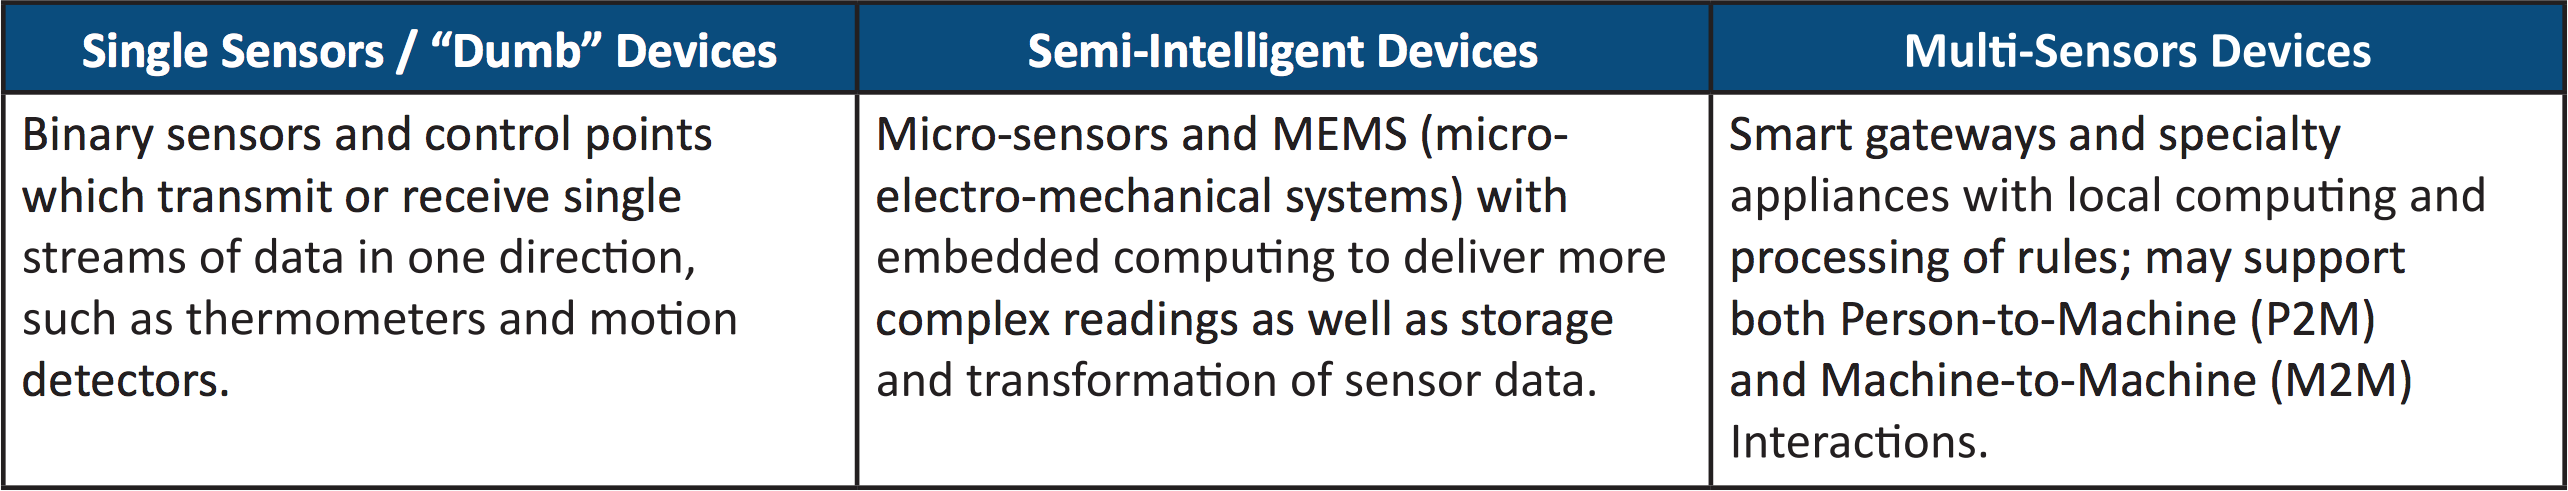
\includegraphics[height=3 cm,keepaspectratio,center]{figures/iotDevices}
	\caption{Unterschiedliche Arten der smarten Objekte \cite{iotdevices}}
	\label{iotdevices}
\end{figure}

\subsubsection{Domain Model}\label{sec:DomainModel}

Da es unter der Buzzword \ac{iot} sehr viele unterschiedlich Auffassungen und Interpretation wie zum Beispiel das ursprüngliche Konzept Kevin Ashtons eines Netzwerkes aus um RFID angereicherter Objekte. Häufig ist auch von \ac{m2m} oder \ac{cps} die Rede. Bei dieser Vielzahl von Auffassungen und Begriffen ist es für ein allgemeines Verständnis unabdingbar sich auf eine Definition zu einigen. Im Zuge dieser Thesis wird das 2010 von Stephan Haller vorgestellte IoT Domain Model verwendet um den Zusammenhang zwischen Devices, Resourcen und Services zu erklären\cite{haller2010things}, da diese die am häufigsten  in der Literatur auf welcher diese Thesis beruht verwendetet wurde. Das Schaubild \ref{domainmodel} zeigt eine auf den Zusammenhang von Device, Service und Ressourcen abstrahierte Darstellung des IoT Domain Models. Im Anhang befindet sich ein Schaubild des vollständigen IoT Domain Models Haller´s vom Stand 2013.

\begin{figure}[H]
	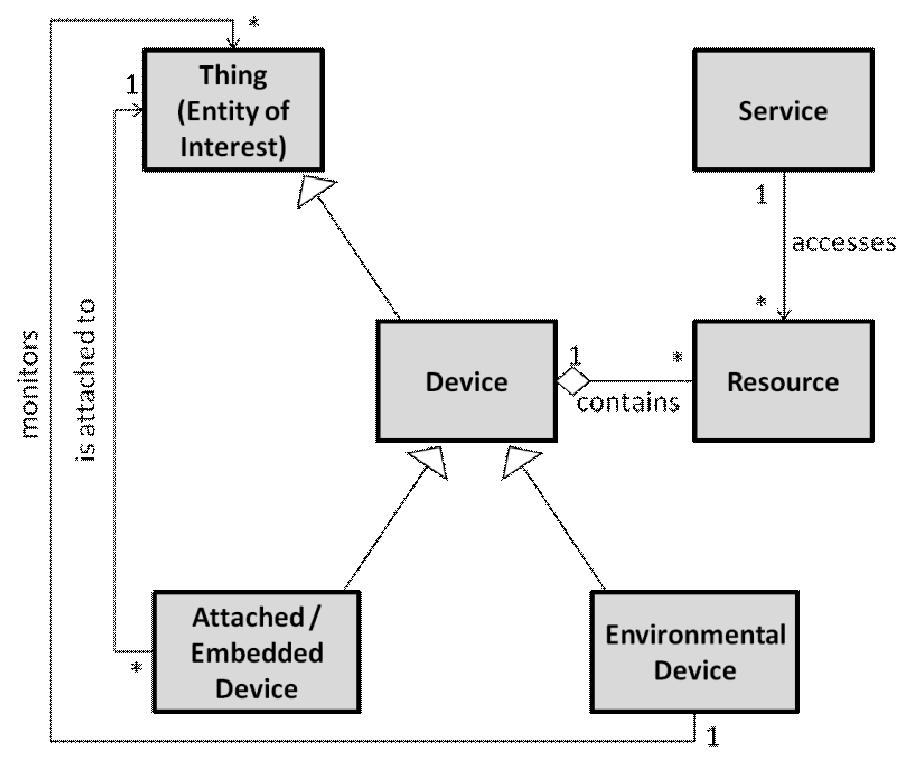
\includegraphics[height=8 cm,keepaspectratio,center]{figures/domainmodel}
	\caption{Zusammenhang zwischen Thing, Device, Resource und Service \cite{haller2010things}}
	\label{domainmodel}
\end{figure}

\textbf{Thing/ \ac{eoi}}: \\ 
Das \ac{eoi} bezeichnet einen physischen Gegenstand an welchem der Nutzer oder eine Anwendung wie zum Beispiel ein Geschäftsprozess. Das \ac{eoi} wird entweder durch ein Environmental Device oder über ein "attached" beziehungsweise "embedded device" überwacht.
\\

\textbf{environmental Device}: 
Environmental Devices, also Umgebungsgeräte überwachen und verfolgen den Status des \ac{eoi}. Beispiele für Umgebungsgeräte sind \ac{rfid} Lesegeräte, Barcodescanner oder Kameras

\textbf{attached/ embedded Device}: 
Als attached/embedded Device stellen ähnlich wie die Umgebungsgeräte den Zustand und den Status des \ac{eoi} fest. Der Unterschied liegt hierbei daran, dass die attached/embedded Devices am \ac{eoi} selbst und nicht in der Umgebung angebracht sind. Beispiel hierfür sind Sensoren wie Thermometer oder Manometer.
\\

\textbf{Device}: \\
Das Device wird als Überklasse der "environmental Devices" sowie der "attached/ embedded Device" verstanden es sammelt also Informationen über das \ac{eoi} und stellt diese über die Möglichkeit der Kommunikation mit IT-Systemen zur Verfügung.
\\

\textbf{Resource}: \\
Als werden die vom Device bereitgestellten digitalen Informationen über den Zustand oder die Betätigungsfähigkeiten eines physischen Objektes bezeichnet.
\\

\textbf{Service}: \\
Services stellen die Ressourcen des Devices über eine klar definierte und standardisierte Schnittstelle bereit und stellen sie somit Anwendungen oder anderen Services zur Verfügung. Somit wird die Funktionalität als Arbeitseinheit einem Geschäftsprozess zur Verfügung gestellt.
\\
\\
Zusammenfassend lässt sich der Zusammenhang zwischen \ac{eoi}, Device, Service und Resource also wie folgend beschreiben. Ein physisches Objekte an welchem Interesse besteht wird durch die Überwachung mittels ein oder mehrerer Sensoren beziehungsweise Umgebungsgeräten als Device in der virtuellen Welt dargestellt. Dieses Device enthält mehrere Ressourcen also Informationen welche wiederum durch standardisierte Schnittstellen, den Services zur Verfügung gestellt werden.

\subsection{Prozessmodellierung}\label{modellierung}

In heutigen Unternehmen unterstützen Informationssysteme nicht mehr nur das Geschäft,sondern sie sind ein integraler Bestandteil davon. Unternehmen machen Gebrauch von Informationstechnologie, und es ist wichtig, dass ihre Systeme so aufgebaut sind, dass sie die Unternehmen unterstützen in denen sie zum Einsatz kommen. Das Geschäft bestimmt letztlich die Anforderungen, welche die Informationssysteme definieren. Die Entwicklung von Software ohne ein angemessenes Verständnis des Kontextes, in welchem diese Software betrieben werden soll, ist nahezu unmöglich. Um ein solches Verständnis zu erlangen, ist es unerlässlich, dass man ein Geschäftsmodell definiert.\\
 Ein Modell ist eine vereinfachte Sicht auf eine komplexe Realität. Diese Abstraktion erlaubt es irrelevante Details zu vernachlässigen und den Fokus auf die Kernelemente zu legen. Effektive Modelle erleichtern zudem
Diskussionen zwischen verschiedenen Stakeholdern im Unternehmen. Sie ermöglichen es ihnen, sich auf die wichtigsten Grundlagen zu einigen und auf gemeinsame Ziele hinzuarbeiten.\\
 Die Modellierung von Geschäftsprozessen ist als Mittel zur Analyse und zum Design von Software akzeptiert und etabliert. Die sich ständig weiterentwickelnden Modelle helfen den Entwicklern auch dabei, ihr Denken zu strukturieren und zu fokussieren. Die Arbeit mit den Modellen dient ihnen zum Verständnis für das Geschäft und erhöht dadurch das Bewusstsein für neue Möglichkeiten zur Verbesserung des Geschäfts.

\subsubsection{BPMN}

\ac{bpmn} ist ein Standard für die Geschäftsprozessmodellierung, der eine grafische Notation zur Spezifikation von Geschäftsprozessen in einem \ac{bpd} auf Grundlage traditioneller Flussdiagrammtechniken bereitstellt \cite[S.222]{Aagesen2015}. Das Ziel von \ac{bpmn} ist es, die Geschäftsprozessmodellierung sowohl für technische Anwender als auch für Geschäftsanwender zugänglich zu machen,damit die Geschäftsprozessmodellierung eine Kommunikations- und Automatisierungsgrundlage bildet.\\
 Hierfür wird eine Notation bereitgestellt wird, welche für Geschäftsanwender intuitiv ist und dennoch komplexe Prozesssemantik abbilden kann. Die seit 2011 von der \ac{omg} vorgestellte \ac{bpmn} 2.0-Spezifikation bietet auch Ausführungssemantik sowie das Mapping zwischen den Grafiken der Notation und anderen Ausführungssprachen, insbesondere der \ac{bpel}. \ac{bpmn} ist so konzipiert, dass es für alle Beteiligten leicht verständlich ist. \\
Zu den Anwendern gehören Business-Analysten, welche die Prozesse erstellen und verfeinern, technische Entwickler, die für die Implementierung zuständig sind sowie Führungskräfte welche Prozesse überwachen und verwalten \cite{vonRosing2015433}. Im Anhang befindet sich ein Poster mit einer Übersicht über die wichtigsten Modellierungsmethoden von \ac{bpmn}. \\
\newline
Aufgrund der fehlenden Möglichkeit Flexibilität abzubilden beziehungsweise da nicht alle Möglichen Szenarien bekannt sind oder aufgrund der Kombinatorik nicht modelliert werden können, wurde 2014 von der \ac{omg} ein eigener Standard \ac{cmmn} verabschiedet welcher in der Lage ist flexible Prozesse abzubilden.\\
 Als Case werden eine Aktivitäten bezeichnet, welche sich nicht exakt wiederholen lässt. Cases sind von sich entwickelnden Umständen oder von Ad-hoc-Entscheidungen im Bezug auf bestimmte Situationen abhängig. Diese Ad-hoc-Entscheidungen werden von sogenannten Wissensarbeitern gefällt.\\
 Zu den Anwendungsfällen des Case Managements gehören die Antrags- und Schadensbearbeitung in der Versicherungsbranche, die Patientenversorgung sowie die medizinische Diagnose im Gesundheitswesen, Hypothekenbearbeitung im Bankwesen, Problemlösung in Call Centern, Wartung und Reparatur von Maschinen und Anlagen sowie die Konstruktion von Sonderanfertigungen\cite{cmmnomg} . \\
Laut Heise sei die Kombination von \ac{cmmn} und \ac{bpmn} sinnvoll um sowohl strukturierte als auch unstrukturierte Prozesse oder Teilprozesse sinnvoll abbilden zu können \cite{cmmnheise}.


\subsubsection{UML}

 \ac{uml} ist eine grafische Sprache, die die Artefakte verteilter Objektsysteme visualisiert, spezifiziert, konstruiert und dokumentiert \cite{Kleuker}. Es ist der am weitesten verbreitete Standard für Software-Architekten, um Geschäftsanwendungen zu spezifizieren.\\
 \ac{uml} wird vor allem für die objektorientierte Softwareentwicklung im Bereich des Software-Engineerings eingesetzt.
Die \ac{uml} wurde in den 90er Jahren als Modellierungssprache und Methodik zur Unterstützung der objektorientierten Programmierung entwickelt. Im Jahr 1997 wurde es als Standard von der \ac{omg} übernommen. Die ersten Versionen 1.X wurden 2005 durch die neu überarbeiteten Versionen 2.X ersetzt. Seit März 2015 befindet sich UML in der Version 2.5 \cite{omguml}. \ac{uml} bietet im Gegenteil zu \ac{bpmn} mehr als nur die reine Prozessmodellierung und ist ihrer Gesamtheit sehr Umfangreich.\\
Die Spezifikation allein ist über eintausend Seiten lang. Strukturiert wird \ac{uml} in vier Gruppen, den  Strukturdiagrammen, den Architekturdiagrammen, den Verhaltensdiagrammen und den Kommunikationsdiagrammen. \\
Im Zuge dieser Thesis wird \ac{uml} lediglich auf \ac{uml} Aktivitätsdiagramme im Bezug auf Prozessmodellierung eingegangen.

\subsubsection{Geschäftsregeln}

Geschäftsregeln an sich sind keine Modellierungsmethode allerdings lassen Geschäftsprozesse selbst als eine Reihe von Geschäftsregeln darstellen. Die unter bestimmten Bedingungen auszuführenden Aktivitäten und die sie auslösenden Ereignisse können in Beziehung zueinander gesetzt werden, so dass Prozesse auf der Grundlage von Geschäftsregeln beschrieben und ausgeführt werden können.\\
Die Prozessmodellierung mit Geschäftsregeln basiert auf den  ECAA-Regeln durch die drei Konstrukte Ereignis, Bedingung und Aktion sowie alternativer Aktion (Event,Condition,Action,Alternative Action). Diese Art der Modellierung eignet sich jedoch nur für kleine Prozessmodelle und müssen für größere Modelle auf die \ac{eepk} Notation übertragen werden \cite{businessrules}. 

\newpage

\section{IoT Workflows und deren Besonderheiten}	%TODO Zusammenhang von IoT und Business Process Modelling, warum ist das schwierig bzw. wichtig?
In diesem Kapitel sollen grundlegende Muster in \ac{iot} Workflows erkannt werden. Anhand der Muster werden Unterschiede zu regulären Workflows gezogen welche im Anschluss zu Anforderungen an die Modellierung von \ac{iot} Workflows zusammengefasst werden. \\

Als Workflow wird eine inhaltlich abgeschlossene sowie zeitlich und sachlich Zusammenhängende Folge von Funktionen bezeichnet. Durch den Workflow werden die Aufgaben, Verarbeitungseinheiten sowie deren Beziehungen zu einander festgelegt \cite{workflowgabler}. Der Workflow kann also als die informationstechnische Umsetzung eines Geschäftsprozesses verstanden werden. \\
Der Lebenszyklus eines Worklows besteht aus der Modellierung, der Ausfürung und Überwachung sowie der Analyse des Workflows. Die Modellierung bildet hierbei den ersten Schritt für die Umsetzung von Workflows, dies geschieht durch einen der in \ref{modellierung} vorgestellten Standards der Geschäftsprozessmodellierung. Diese Thesis beschränkt sich auf den Modellierungsaspekt des Workflow Lebenszykluses.
%Wie in Problemstellung angesprochen komplexere Prozesse können durch viele Zusammengefasste IoT Subprocesses dargestellt werden(Industrie 4.0). Diese Subprocesses entsprechen dem geforderten micro processes
%Mögliches Problem, Darstellung von Streams. Mögliche Lösung Time based Subprocesses mit IoT A modelliert,ermöglicht genaue zuweisung und nachverfolgung von IoT Device zu physical Entity -> wichtig für automatisierung (workflow). \\

%Umsetzung von IoT A BPMN in Workflow/BPMN Engine deliverable 2.3 wichtig !

%Eventuell neuer Punkt Umsetzung der BPMN Erweiterung (Vollständiges UML Erweiterungsdiagramm lässt sich in XML darstellen und in BPMN integrieren)

\subsection{Typische Muster von IoT Workflows} \label{iotmuster}

Da das \ac{iot} eine noch sehr junge Technologie ist und sich größtenteils im experimentellem Stadium befindet existieren weitestgehend keine Best Pracitices. Durch die Analyse gängiger Use Cases und Geschäftsmodelle \cite{iotbusinessmodels} des \ac{iot} wurden daher die folgenden Muster als Kern Workflows herausgearbeitet.

Muster 1: Simpler \ac{iot} Worflow\\
Ein oder mehrere IoT Devices (Sensoren) überwachen den Zustand beziehungsweise Standort einer \ac{eoi}. Die Daten selbst können vom IoT Device ausgewertet werden. Je nach Auswertung der Daten kann das Device andere Devices ansprechen welche Tätigkeiten ausführen die den Zustand der \ac{eoi} verändern.
 
Muster 2: Komplexer \ac{iot} Workflow\\
Die von den \ac{iot} Devices gesammelten Daten können nicht einfach ausgewertet werden sondern müssen an externen System mitgeteilt werden,welcher in der Lage ist die Daten auszuwerten. Je nach Auswertung der Daten ist dieses System in der Lage dazu andere Devices anzusprechen welche den Zustand des \ac{eoi} ändern können. 

%TODO Name für Muster finden
Muster 3: Verwendung der \ac{iot} Daten für neuen Geschäftsprozess \\ 
Durch \ac{iot} Devices werden große Mengen an Daten gesammelt. Diese Daten dienen dazu völlig neue Geschäftsmodelle zu kreieren wie zum Beispiel pay per Use. Hierbei können die von den IoT Device generierten Daten mittels Big Data Technologien wie maschinellem Lernen und Complex Event Processing verwendet werden um aus den Datenmengen höherwertige Informationen und Ereignisse zu generieren. \\

Prozesse können aus ein oder mehreren Mustern zusammengesetzt werden.  

Aufgrund der geringen Rechenleistung wird teilweise Backend für die Auswertung der Daten benötigt -> Orchestration. Bei einfacheren Tasks ist Choreographie sinnvoll (Brauerei Beispiel). Herangehensweise von Rechenleistung abhängig, wenn die Auswertung der Daten zu komplex für embedded Device ist wird ein Backend benötigt (Orchestration). In folge dessen. Die Modellierung muss hier die Möglichkeiten der Technik berücksichtigen. 

\subsection{Unterschiede IoT Workflows zu regulären Workflows}

Aus den in \ref{iotmuster} definierten Mustern von \ac{iot} Workflows lassen sich die \ac{iot}-spezifischen Unterschiede gegenüber regulärer Workflows ableiten. 

Der grundlegendste Unterschied von \ac{iot} Workflows liegt darin, dass \ac{iot} Devices einen neuen Akteur im Workflow darstellt, welcher Tätigkeiten ausführen und mit anderen Prozessteilnehmern sowie weiteren \ac{iot} Devices kommunizieren kann. \\
Devices unterscheiden sich in ihren Eigenschaften von regulären Prozess Teilnehmern, sie können fest verbunden sein mit den Entitäten mit welchen sie zusammen arbeiten. Ein Device muss sich also ein oder mehrerer Entität zuweisen lassen. Diese Abhängigkeit ist bei der Modellierung zu berücksichtigen. \\
Durch die Verbundenheit von \ac{iot} Devices besitzen diese auch eine eigene Form mit Dingen innerhalb eines Prozesses zu interagieren, da ihre Handlungen sich im Kern auf den Zustand der ihr zugewiesen Entität beschränken.\\
Da sich die Entitäten innerhalb der Workflows bewegen können spielt Mobilität sowie die Fähigkeit den Standort der \ac{iot} Devices und Entitäten bestimmen zu können eine besondere Rolle in \ac{iot} Workflows\\
Die von den \ac{iot} Devices gesammelten Informationen unterscheiden müssen Metadaten darüber enthalten wann sie wo von welchem \ac{iot} Device über welche Entität gesammelt wurden sowie Aufschluss über die Qualität der Information selbst beinhalten um eine sinnvolle Auswertung der Informationen selbst zu ermöglichen.



\subsection{IoT Spezifische Anforderungen an die Modellierung}
 
\section{Betrachtung verschiedener Modellierungsansätze}
Obwohl IoT mittlerweile zum beliebten Schlagwort geworden ist, existieren immer noch Probleme mit dem Konzept, Prozesse auf \ac{iot} anzuwenden und diese fachgerecht darzustellen. In diesem Kapitel werden deshalb verschiedene Modellierungsansätze vorgestellt, welche auf die Besonderheiten von \ac{iot} Workflows spezialisiert sind.

\subsection{IoT - A}

\acl{iota} kann als eine Art Leuchtturmprojekt der Europäischen Union angesehen werden, welches 2013 nach über drei Jahren zu Ende ging. Ziel hierbei war es ein \ac{arm} als Grundlage für das \ac{iot} zu erstellen. Die Grundidee hierbei war, dass das \ac{arm} eine gemeinsame Struktur sowie Richtlinien für den Umgang mit Kernaspekten der Entwicklung, Nutzung und Analyse von \ac{iot}-Systemen bereitstellt, was eine nahtlose Integration heterogener \ac{iot}-Technologien in eine kohärente Architektur sowie den Zusammenschluss mit anderen Systemen des "Future Internet" ermöglicht \cite[S.17]{enablingthingstotalk}. Um dieses Ziel zu erreichen wurden einige detaillierte wissenschaftliche und technologische Zielsetzungen identifiziert welche innerhalb des Projektes behandelt werden\cite{meetiot}.
\newline

\textbf{Zielsetzungen}
\\

1. Bewertung bestehender IoT-Protokoll Suites und Ableitung von Mechanismen zur Erzielung einer durchgehenden Interoperabilität für eine nahtlose Kommunikation zwischen IoT-Geräten. Das IoT wird aus Geräten mit unterschiedlichen Kommunikationsstacks bestehen. \ac{iota} soll eine nahtlose Kommunikationsfluss zwischen heterogenen Geräten ermöglichen und dabei die Komplexität der End-to-End-Heterogenität vor dem Kommunikationsdienst verbergen.
\\

2. Entwicklung von Modellierungswerkzeugen und einer Beschreibungssprache für zielorientierte \ac{iot}-bewusste (Geschäfts-)Prozessinteraktionen, die es erlauben, ihre Abhängigkeiten für eine Vielzahl von Bereitstellungsmodellen auszudrücken.
\\

3. Ableitung von adaptiven Mechanismen für die verteilte Orchestrierung von \ac{iot}-Ressourcen-Interaktionen, die Selbst-*-Eigenschaften freilegen, um mit der komplexen Dynamik realer Umgebungen umzugehen. 
\\

4. Ganzheitliche Einbettung effektiver und effizienter Sicherheits- und Datenschutzmechanismen in \ac{iot}-Geräten sowie den von ihnen genutzten Protokollen und Diensten.
\\

5. Entwicklung einer neuartigen Auflösungsinfrastruktur (resolution infrastructure) für das \ac{iot}, die es ermöglichen soll, ein skalierbares zuweisen von \ac{iot}-Ressourcen, Entitäten der realen Welt und ihrer Assoziationen durchzuführen.
\\

6. Entwicklung von IoT-Geräteplattformkomponenten einschließlich der Gerätehardware und Laufzeitumgebung. Das \ac{iota} soll Schlüsselkomponenten entwickeln, die für die \ac{iot}-Geräteplattform erforderlich sind, auf der ein zukünftiges Internet der Dinge basieren wird. 
\\

7.Der Verbreitung und Nutzung der entwickelten architektonischen Grundladen beizutragen.
\\

Im Zuge dieser Thesis ist besonders das Ziel der Entwicklung von Modellierungswerkzeugen sowie einer Beschreibungssprache für zielorientierte \ac{iot} bewusste Prozessinteraktionen von Bedeutung auf welches im folgenden Kapitel genauer eingegangen wird. 

\subsubsection{IoT- A Modellierunskonzept}
Innerhalb des \ac{iota} Projektes wurde ein Modellierungskonzept für \ac{iot} Prozesse entworfen. Dieses sogenannte \ac{iapmc} stellt eine Erweiterung um neue Elemente dar welche sich in \ac{bpmn} integrieren lassen  \cite{conceptsiotawarepm}. Diese Elemente werden im folgenden vorgestellt
\newline

\textbf{1.1. Actuation Activity}
\newline
Als Aktuator wird ein physisches Bauteil bezeichnet welches elektronische Signale in mechanische Bewegungen oder andere physikalische Auswirkungen umsetzen kann. Ein Aktuator führt also Tätigkeiten ganz oder nach vorgegeben Werten aus. Nach der erfolgreichen Durchführung einer "Actuation Activity" hat sich also der physische Zustand eines physischen Gegenstandes geändert.\\
Innerhalb des \ac{iot} erfolgt die Interaktion mit den Softwarekomponenten solcher Aktoren durch Services innerhalb konkreter Prozesse, die über klar definierte Serviceschnittstellen verfügen.\\
Funktionelle Eigenschaften der Actuation Activity sind, dass es einen Input Datensatz gib, jedoch keinen Output Datensatz. Es weder durch die Business Process Execition Engine gestartet noch gemanaged wird. Es besitzt eine genau definierte Schnittstelle und eine Verbindung zu einem Data Object beziehungsweise einem Data Store. Stellt einen Service bereit mit welchem der Zustand der physischen Entity geändert wird \cite[S.41]{conceptsiotawarepm}. In Abbildung \ref{fig:actuationtask} ist das fertige Model einer "Actuation Task" nach \ac{iapmc} zu sehen.

\begin{figure}[H]
	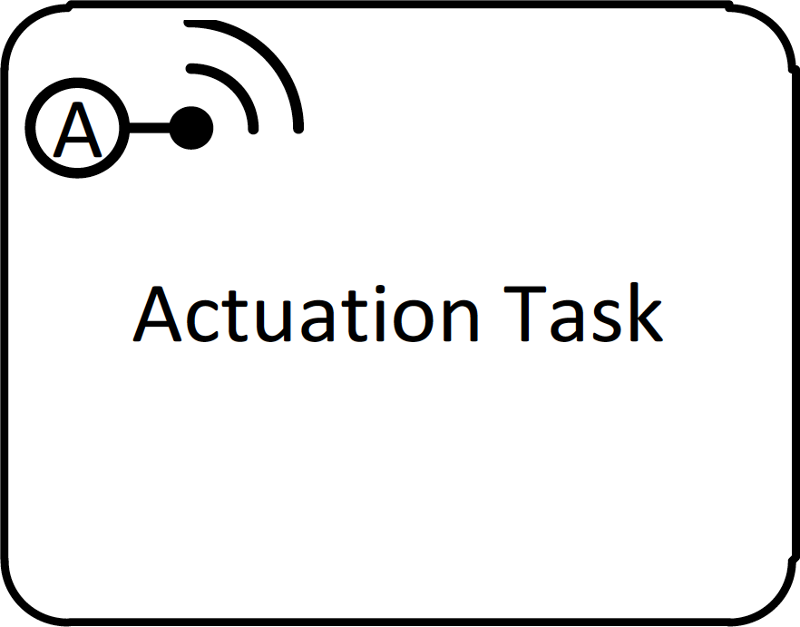
\includegraphics[height=2 cm,keepaspectratio,center]{figures/ActuationTask}
	\caption{Actuation Task \cite[S.44]{conceptsiotawarepm}}
	\label{fig:actuationtask}
\end{figure} 

\textbf{1.2. Sensing Activity}
\newline
Sensoren sind physische Elemente welche Bewegungen oder physikalische Werte erfasst und in elektronische Singale umwandelt. In der \ac{iot} Welt ist ein Sensor in der Lage den Zustand einer phsischen Entität zu erfassen, dieses Erfassen des physischen Zustandes wird als "sensing" bezeichnet.\\
Sensoren sind in gewisser Weise als Gegenstück zu den Aktoren zu verstehen, ein Aktor ändert den Zustand einer physischen Entität während der Sensor seinen Zustand misst und somit die Änderung seines Zustandes registrieren kann. Als Gegenstück zu den Aktoren haben "Sensing Activities" keinen Daten Input aber dafür einen Daten Output. Allerdings werden auch diese weder weder durch die Business Process Execition Engine gestartet noch gemanaged sondern werden durch eine standardisierte Schnittstelle bereitgestellt und besitzen Anbindung an ein Data Object beziehungsweise Store \cite[S.45]{conceptsiotawarepm}. Der in Abbildung \ref{fig:sensingtask} ersichtliche Sachverhalt stellt den von der \ac{iapmc} entwickelten "Sensing Task" dar.

\begin{figure}[H]
	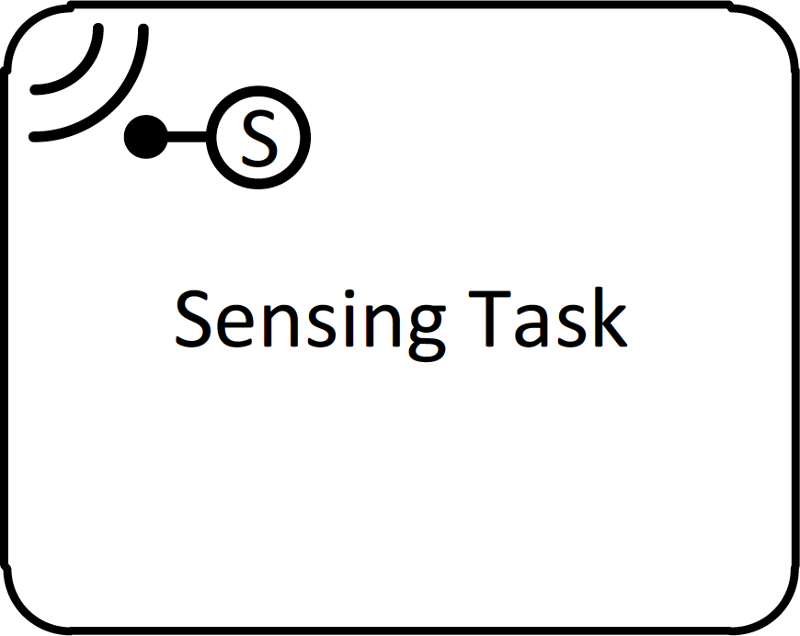
\includegraphics[height=2 cm,keepaspectratio,center]{figures/SensingTask}
	\caption{Sensing Task \cite[S.49]{conceptsiotawarepm}}
	\label{fig:sensingtask}
\end{figure} 

\textbf{3. IoT Device}
\newline
Wie in \ref{sec:DomainModel} beschrieben besitzt ein \ac{iot} Device die Fähigkeit den Status einer \ac{eoi} wahrzunehmen und mit einem Netzwerk zu kommunizieren. Des weiteren besitzt ein \ac{iot} Device im \ac{iota} Kontext die Möglichkeit aktiv den Status seiner physischen Entität oder einer anderen im \ac{iot} vorhandenen Netzwerk zu verändern. Mobiltelefone, ein Sensor-Knotenpunkt, einzelne Sensoren oder Aktuatoren sind Beispiele für ein \ac{iot} Device \cite[S.50]{conceptsiotawarepm}. Jeder Aktuator oder Sensor kann demnach als \ac{iot} Device angesehen werden. Hinzu kommt, dass \ac{iot} Devices Parameter besitzen welche die automatische Zuweisung durch die Auflösungsinfrastruktur anpassen und deren Verwendbarkeit bestimmen. \\
Wie in Abbildung \ref{fig:iotdevice} zu sehen ist das \ac{iot} Device, in diesem Fall ein Mobiltelefon, ein eigenständiger Akteuer und besitzt eine eigene Swimlane. Durch das Aufklappen lassen sich die Parameter der Spezifikation anzeigen.

\begin{figure}[H]
	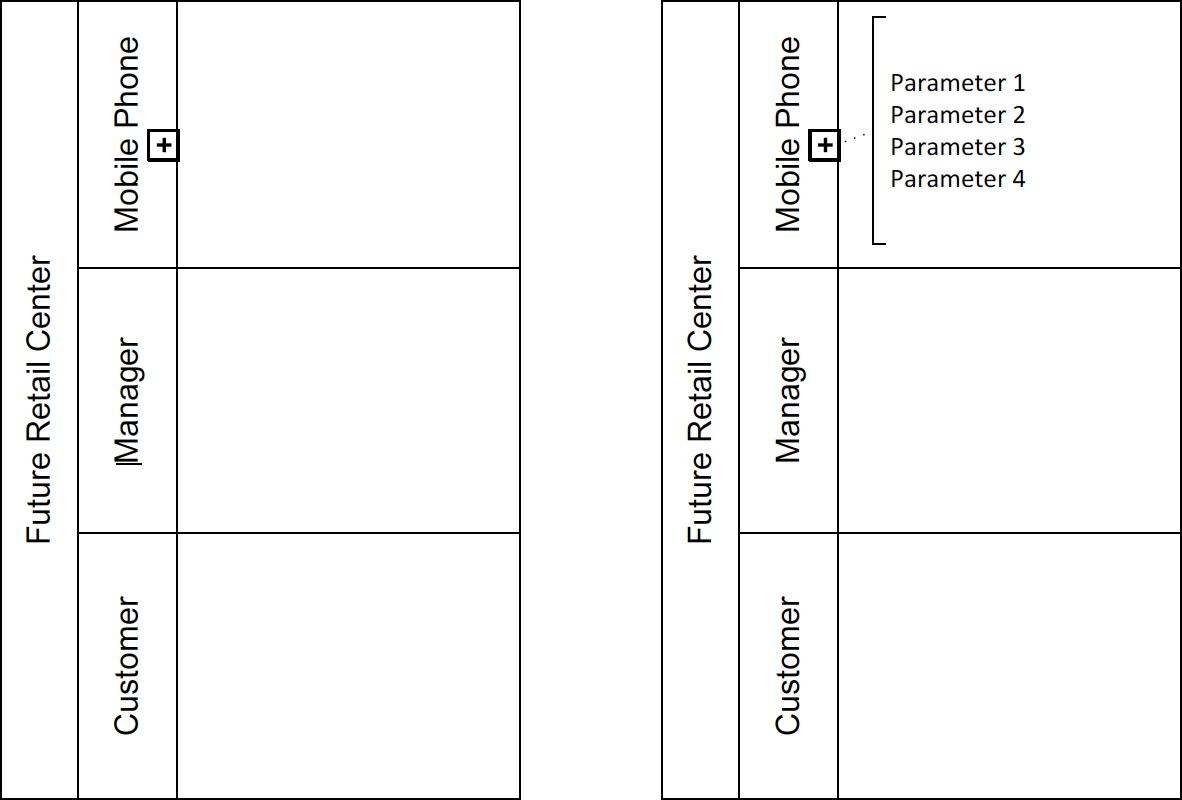
\includegraphics[height=7 cm,keepaspectratio,center]{figures/IoTDevice}
	\caption{IoT Device \cite[S.53]{conceptsiotawarepm}}
	\label{fig:iotdevice}
\end{figure} 

\textbf{4. Process Resources}
\newline
Die Definition von Ressourcen des \ac{iapmc} unterscheidet sich von der in \ref{sec:DomainModel} vorgestellten. Demnach seien Ressourcen in der Geschäftsprozessmodellierung ein abstraktes Konzept welches zur Klassifizierung der menschlichen oder technischen Einsatzfähigkeit während der Prozessauflösung für die Ausführung diene. So könne eine Ressource mehrere Aktivitäten ausführen und Aktivitäten könnten mehrere Ressourcen verwenden. Ein Beispiel für eine Ressource in der Prozessmodellierung ist ein IoT-Gerät wie ein Temperatursensor, der Messmöglichkeiten in Form von Prozessaktivitäten für die Prozessausführung bereitstellen kann\cite[S.54]{conceptsiotawarepm}. Eine Resource entspricht also einem Pool in \ac{bpmn} muss allerdings noch um Parameter für die Zuweisung sowie Metainformationen ergänzt werden.
\\

\textbf{5. Physical Entity}
\newline
Als Physical Entity also eine physische Entität wird ein Objekt aus der physischen Welt welches relevant für einen Benutzer oder eine Anwendung ist. Deshalb fällt in diesem Zusammenhang auch häufig der Begriff \acl{eoi} als ein Objekt an welchem Interesse besteht. Physische Instanzen in einem Prozess können für eine oder mehrere Aktivitäten relevant sein. Geschäftsprozesse gehen oft über Abteilungs- und Betriebsgrenzen hinweg, die sich in einem Prozess mit Hilfe von Pools und Lanes abbilden lassen. Physikalische Einheiten können innerhalb dieser Abteilungs- und Einsatzgrenzen existieren, aber auch darüber hinausgehen. Des weiteren können physische Entitäten für eine oder mehrere \ac{iot} Devices relevant sein\cite[S.58-59]{conceptsiotawarepm}. Physische Entitäten besitzen genauso wie \ac{iot} Devices Parameter die für die automatische Zuweisung von \ac{iot} Devices zu den physischen Entitäten relevant sind. Wie in Abbildung \ref{fig:physicalentity} zu sehen lassen sich Physical Entitys ebenso aufklappen um die Parameter anzeigen zu lassen wie die \ac{iot} Devices in Abbildung \ref{fig:iotdevice}. 

\begin{figure}[H]
	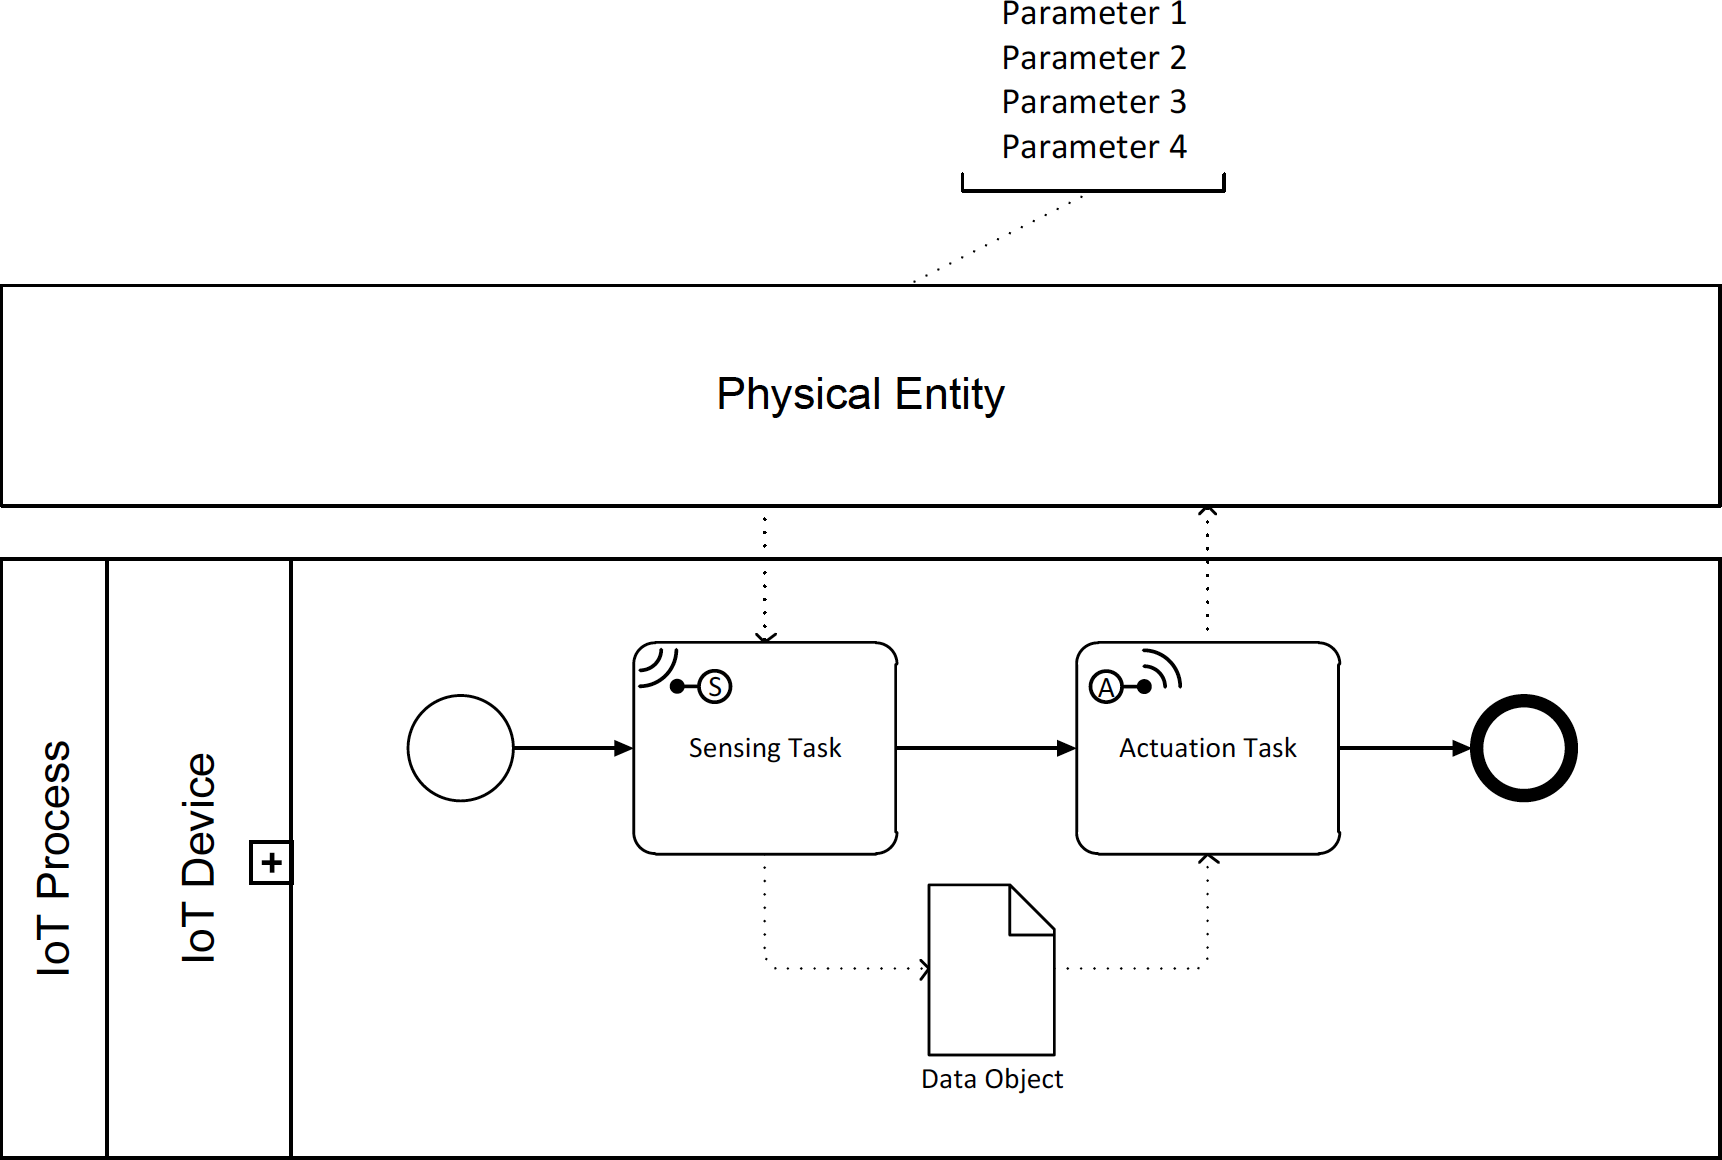
\includegraphics[height=7.3 cm,keepaspectratio,center]{figures/PhysicalEntity}
	\caption{Physical Entity \cite[S.62]{conceptsiotawarepm}}
	\label{fig:physicalentity}
\end{figure} 

\textbf{6. Real World Data Object / Store}
\newline
Ein Real-World Data Object stellt ein temporär gespeichertes Datenobjekt einer laufenden Prozessinstanz dar, das durch die Messung eines IoT Devices erzeugt wurde. Die Werte des Datenelements sind für andere Prozessbeteiligte sichtbar und existieren nicht über die Lebensdauer eines Prozesses hinaus. Das Real-World Data Object hat IoT-spezifische Eigenschaften, wie z.B. die unterschiedliche Qualität der Informationen. Neben einem Real-World Data Object kann ein Geschäftsprozess auch einen Real-World Data Store enthalten. Im Gegensatz zum Real-World Data Object stellt der Real-World Data Store persistente Daten dar und existiert über die Lebensdauer einer Prozessinstanz hinaus. Der Real-World Data Store kann von den Teilnehmern des Prozesses sowie von Teilnehmern außerhalb des Prozesses abgefragt oder aktualisiert werden. Real-World Data Objects sowie Real-World Data Stores besitzen Eigenschaften welche darüber Auskunft erteilen wann welches \ac{iot} Device den Datensatz über welche Physische Entität erstellt hat \cite[S.64-65]{conceptsiotawarepm}. In Abbildung \ref{fig:datastore} und \ref{fig:datastore} sind die Modelle mehrerer Data Objects beziehungsweise Data Stores mit ausgeklappten Eigenschaften zu sehen.

\begin{figure}[H]
	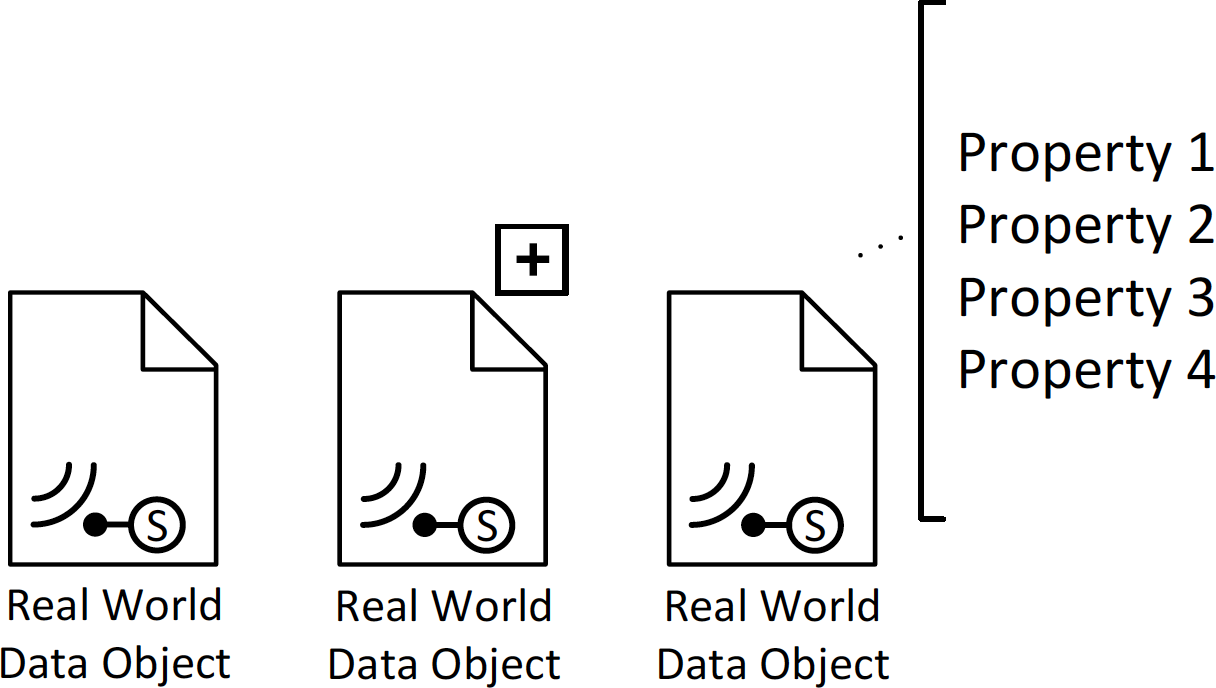
\includegraphics[height=3.5 cm,keepaspectratio,center]{figures/DataObject}
	\caption{Data Object \cite[S.67]{conceptsiotawarepm}}
	\label{fig:dataobject}
\end{figure} 

\begin{figure}[H]
	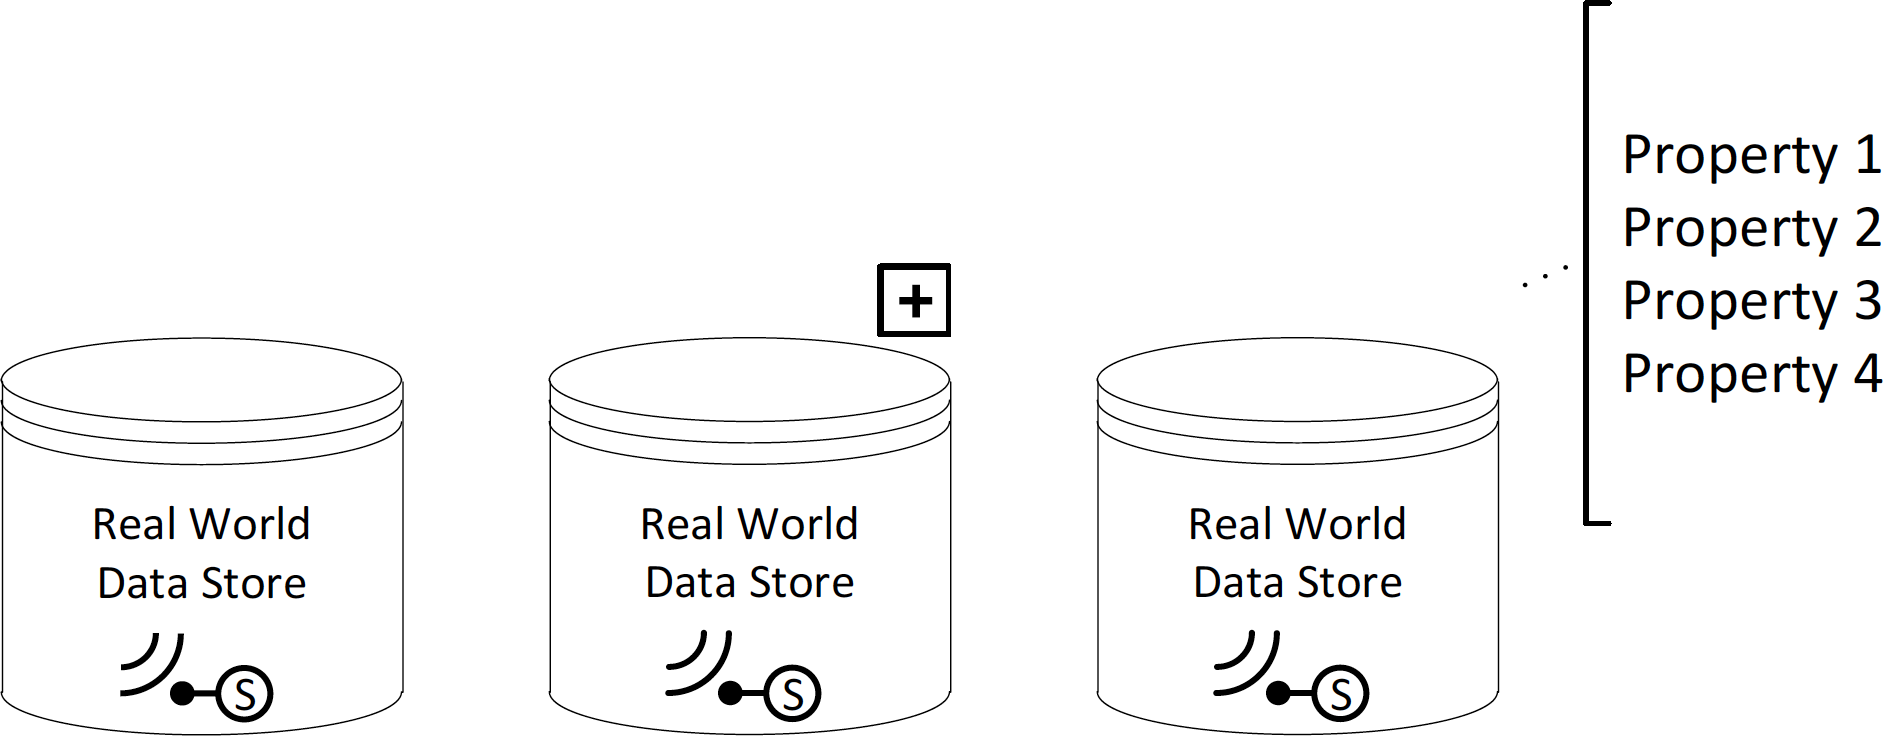
\includegraphics[height=3 cm,keepaspectratio,center]{figures/DataStore}
	\caption{Data Store \cite[S.67]{conceptsiotawarepm}}
	\label{fig:datastore}
\end{figure} 

\textbf{6. Mobility Aspect}
\newline
Mobilität kann Prozessbeteiligte wie IoT Devices oder die Physical Entitys betreffen, welche dadurch die Aktivitäten beeinflussen, für die sie verantwortlich sind. Dieser Aspekt bezieht sich sowohl auf IoT-Aktivitäten als auch auf normale Aktivitäten. In Folge dessen werden Prozesse oder Teilprozesse durch das mobile Verhalten ihrer "Teilnehmer", also deren Ortswechsel beeinflusst. So können Prozesse aufgrund von dem Erreichen eines \ac{eoi} an einem bestimmten Ort oder der signifikanten Lageänderung ausgelöst werden beziehungsweise Abhängig davon sein. Deshalb benötige \ac{bpmn} Erweiterungen um zu Kennzeichnen wenn ein Prozess, ein Prozessteilnehmer, eine Prozessentscheidung oder eine Aktivität mobil seien \cite[S.68-70]{conceptsiotawarepm}. Das in Abbildung \ref{fig:mobile} auf der linken Seite zu sehende Symbol indiziert, dass die Komponente in welcher sie verwendet wird mobil ist während das rechte Symbol die Ortsabhängigkeit darstellt.

\begin{figure}[H]
	
\includegraphics[height=0.75 cm,keepaspectratio,center]{figures/Mobile}
	\caption{Mobile Property, Location based Property\cite[S.71]{conceptsiotawarepm}}
	\label{fig:mobile}
\end{figure} 

Zusammengefasst lässt sich das \ac{iota} Modellierungskonzept an dem in Abbildung \ref{fig:iotaprocess} veranschaulichen. Hierbei geht es um einen Sensor basierten Qualitätskontrollprozess. Eine Orchidee ist hierbei die Physische Entität welche mittels eines smarten Temperatur Sensors überwacht wird. Alle 60 Sekunden wird ein sensing Task ausgelöst welcher die Temperatur der Orchidee misst und das daraus resultierende Data Object an ein Backend System weiterleitet. Sofern die Temperatur nicht außerhalb der Norm liegt endet der Prozess. Ansonsten wird sowohl eine Alarm Benachrichtigung auf dem SmartPhone Ted angezeigt, welcher ein mobiler Prozessteilnehmer ist, sowie eine Berechnung des neuen Preises des Backend Systems veranlasst. Der angepasste Preis wird an einen Aktuator, das Regaletikett weitergeleitet, welcher den neuen Preis der Orchidee anpasst und somit den Prozess beendet. In diesem Prozess werden ein Großteil des \ac{iapmc} sinnvoll dargestellt und eingesetzt.

\begin{figure}[H]
	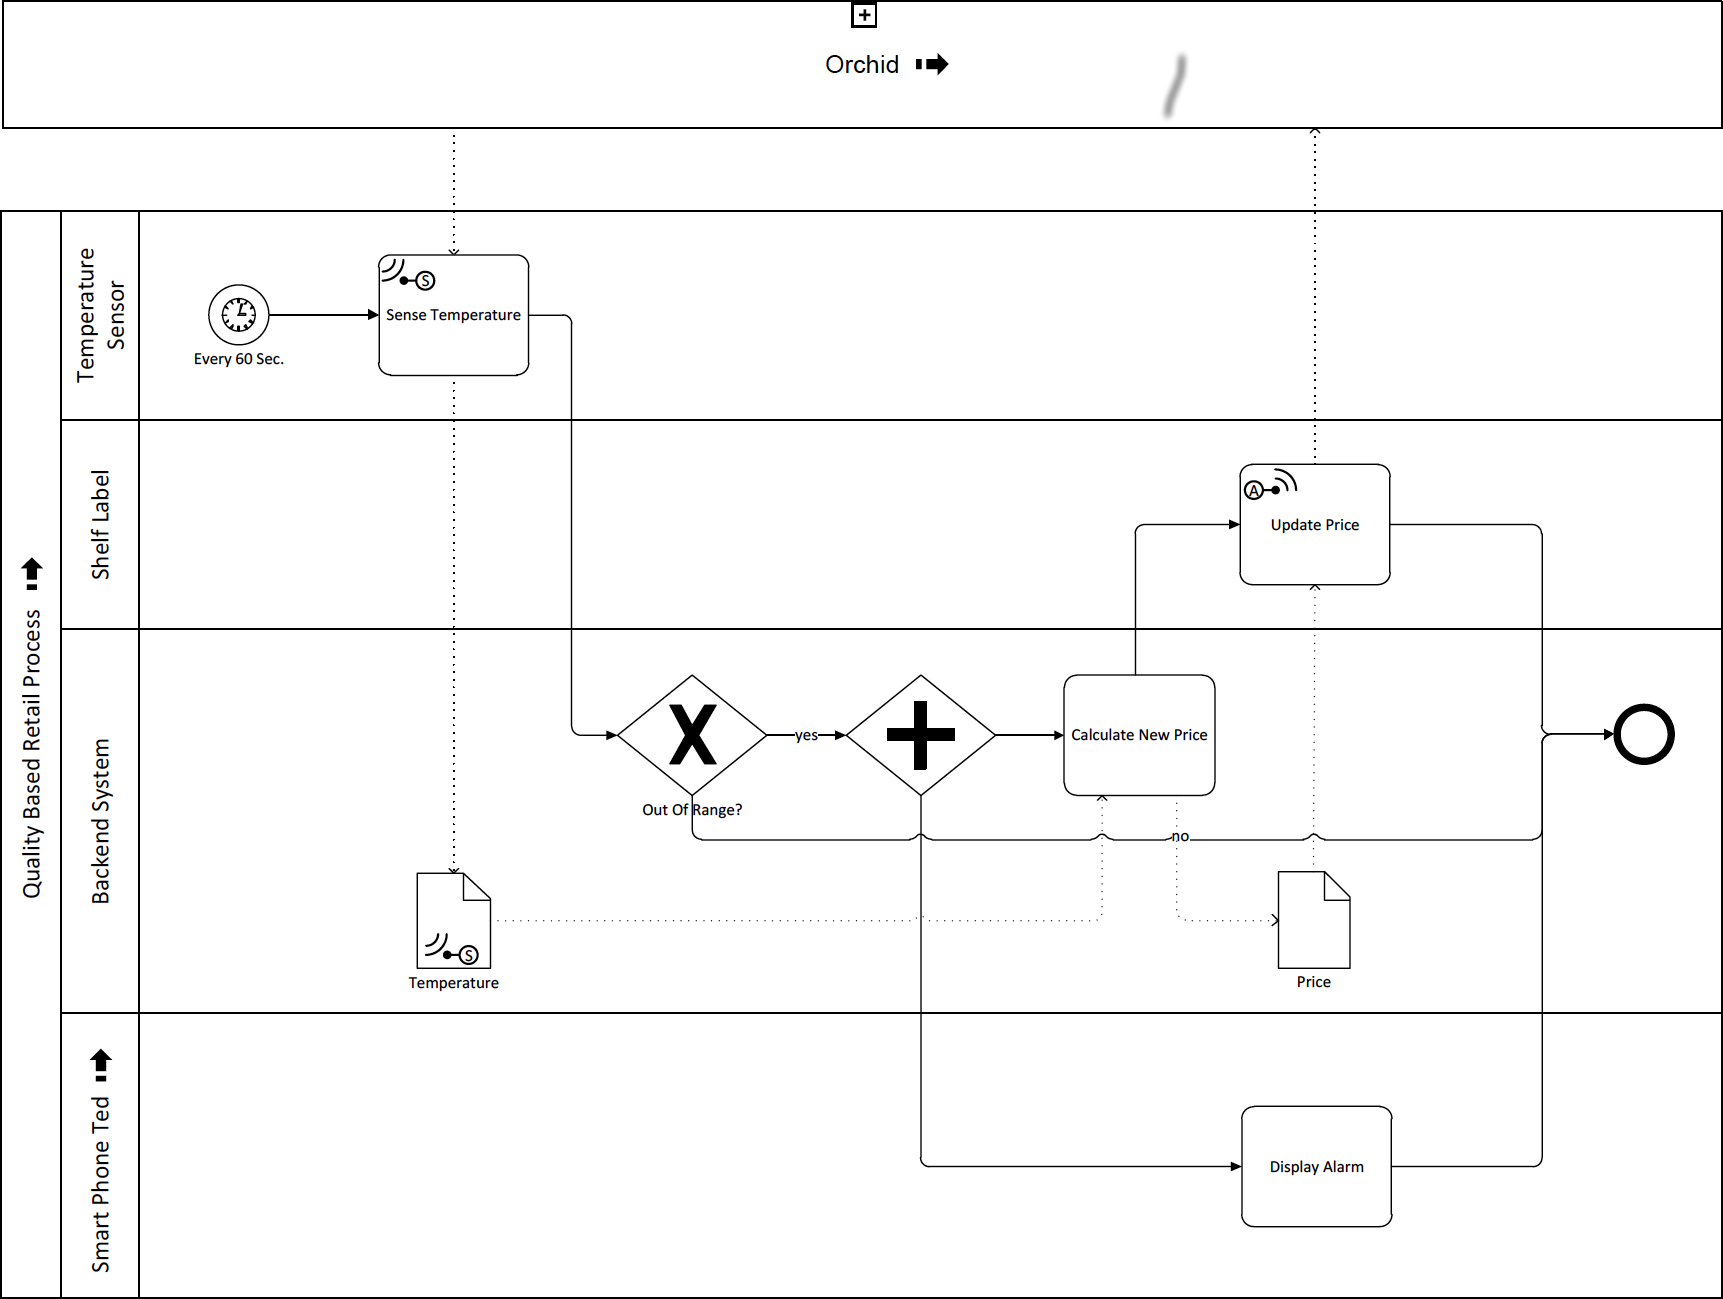
\includegraphics[height=11 cm,keepaspectratio,center]{figures/iotaprocess}
	\caption{\ac{iapmc} Beispiel\cite[S.81]{conceptsiotawarepm}}
	\label{fig:iotaprocess}
\end{figure} 

\subsection{BPMN4CPS} 

\ac{bpmn4cps} stellt ähnlich wie \ac{iapmc} ein Konzept vor welches die \ac{bpmn} um Besonderheiten von \ac{iot} beziehungsweise \ac{cps} erweitern soll. Dieses Konzept wurde erstmalig bei der 25 IEEE Conference on Enabling Technologies: Infrastructure for Collaborative Enterprises vorgestellt. Ziel hierbei ist es den Entwicklern zu ermöglichen, CPS-Elemente, -Konzepte und -Eigenschaften bei der Modellierung von CPS-Prozessen präzise und effizient zu berücksichtigen. Hierfür wurden Relevante Eigenschaften von \ac{cps} herausgearbeitet auf welche im folgenden Abschnitt eingegangen wird.
Die für \ac{cps} relevanten Charakteristiken lauten nach \cite{BMPN4CPS} wie folgt:

\textbf{Aufgaben Typen}
\\
Im physischen Prozess können CPS-Aufgaben eine physische oder eine manuelle Aufgabe sein. Die physische Aktivität liefert Sensordaten oder führt Aktionen aus, die sich auf die physische Welt auswirken. Sie können die Aktivität eines Sensors wie der Temperaturmesssensor oder die Aktivität eines Aktors wie die Luftkühlung durch eine Klimaanlage sein. Während eine manuelle Aufgabe von einem Menschen ohne die Hilfe eines Geräts oder einer Anwendung ausgeführt werden soll
\newline
\textbf{Eintäten-/Resourcen basiertes Konzept}
\\
Das physikalische Gerät hat eine schlechte Rechenleistung und einen dynamischen Zustand. Die Ausführung einer physischen Aktivität kann sich auf die physischen Einheiten und das Gerät auswirken, indem sie ihre lokalen Zustände ändert. Daher müssen während der Modellierungsphase weitere Informationen über die beteiligte Entität, Ressource oder das Device bereitgestellt werden
\newline
\textbf{Event basierte, Befehl/Aktions basierte und periodische Aufgaben}
\\
Eine Aufgabe kann durch ein Ereignis oder eine Befehlsnachricht ausgelöst werden. Es kann auch eine periodische Aufgabe sein, die in jedem Intervall oder zu jedem Zeitpunkt stattfinden soll. Diese Annotationen werden von BPMN unterstützt.
\\
\textbf{Mobilität}
\newline
Das physische Gerät kann mobil oder statisch sein. Diese Eigenschaft ist wichtig, da zusätzliche Informationen beim mobilen Verhalten zur Laufzeit berücksichtigt werden müssen.
\newline
\textbf{Verfügbarkeit}
\\
Eine physische Aktivität kann nur dann einsatzbereit sein, wenn ihr Anbieter zeitlich und räumlich verfügbar ist.
\newline
\textbf{Zeitliche Anforderungen}
\\
Das zeitliche Verhalten ist die zentrale Eigenschaft der physikalischen Prozesse, bei denen die Zeit entscheidend ist. Besonders bei kritischen Anwendungen müssen physikalische Maßnahmen zur richtigen Zeit und zum richtigen Zeitpunkt getroffen werden
\newline
\textbf{Räumliche Eigenschaften}
\\
Sind die Anforderungen, welche mit physischen Aktivitäten verbunden sind. Sie stellen den Ort dar, an dem die Aktivität ausgeführt werden soll, und den betroffenen Bereich, der durch die Aktivität des Sensors beziehungsweise des Aktors beeinflusst werden soll.
\newline
\textbf{Zeit Räumliche Eigenschaften}
\\
Die physische Umgebung ist kontinuierlich dynamisch. Diese Dynamik kann raum-zeitlicher Natur sein, die Zeit- und Rauminformationen kombiniert. Zum Beispiel ändert sich der Zustand eines physischen Objekts kontinuierlich entsprechend seiner Position in Raum und Zeit.
\newline
\textbf{Kontext Eigenschaften}
\\
Der Kontext und die reale Umgebung, in der die physischen Aktivitäten ausgeführt werden, beeinflussen ihr Verhalten. So besteht beispielsweise ein enger Zusammenhang mit der physischen Bewegung eines Fahrzeugs und seiner Umgebung 

\subsubsection{BPMN4CPS Modellierungskonzept}

Für die Umsetzung eines Cyber Physischen Prozesses sind laut des \ac{bpmn4cps} mindestens drei Pools nötig. Der erste Pool stellt den physischen Prozess dar, der zweite Pool den Cyber Prozess und der dritte einen Controller welcher für die Kommunikation zwischen dem Cyber Prozess und dem phyischen Prozess orchestriert. Außerdem wurde der in Abbildung \ref{fig:physicaltask} sichtbaren Physical Task  angelegt. Dieser unterscheidet zwischen einem Actuator's Task und einem Sensor's Task. Ein Actuator's Task nimmt einfluss auf den Zustand einer physical Entity während ein Sensor's Task dessen Zustand misst.

\begin{figure}[H]
	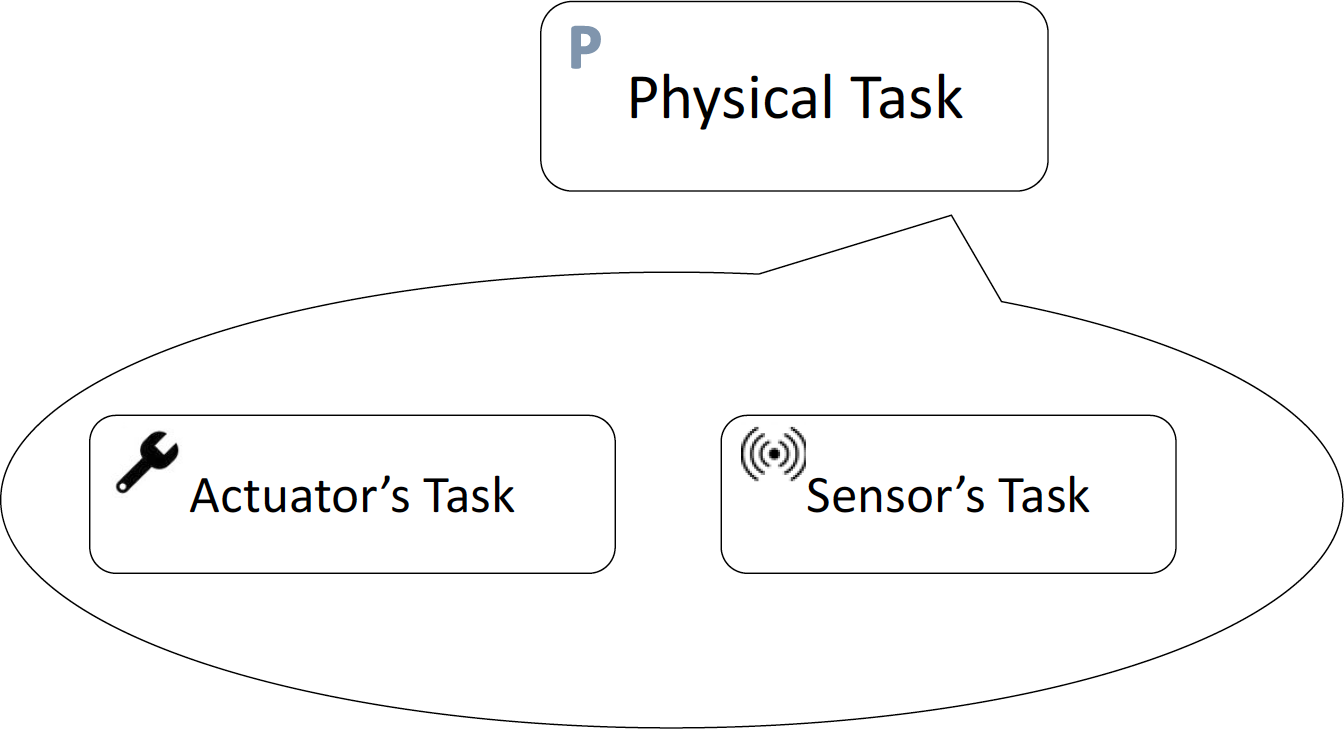
\includegraphics[height=4 cm,keepaspectratio,center]{figures/PhysicalTask}
	\caption{Physical Task\cite{BMPN4CPS}}
	\label{fig:physicaltask}
\end{figure} 

Des weiteren wurde der in Abbildung \ref{fig:cybertask} zu sehende Cyber Task angelegt welcher eine Erweiterung des schon in \ac{bpmn} bestehenden Service Task darstellt. Dieser Task besitzt drei Ausführungen den Embedded Service Task, welcher einen Cyber Task darstellt der an einem \ac{iot} Device selbst ausgeführt wird, den Web Serice Task, bei dem die Aufgabe an einen Webservice weitergeleitet wird und den Cloud Service Task welcher von einem Cloud Service ausgeführt wird.  

\begin{figure}[H]
	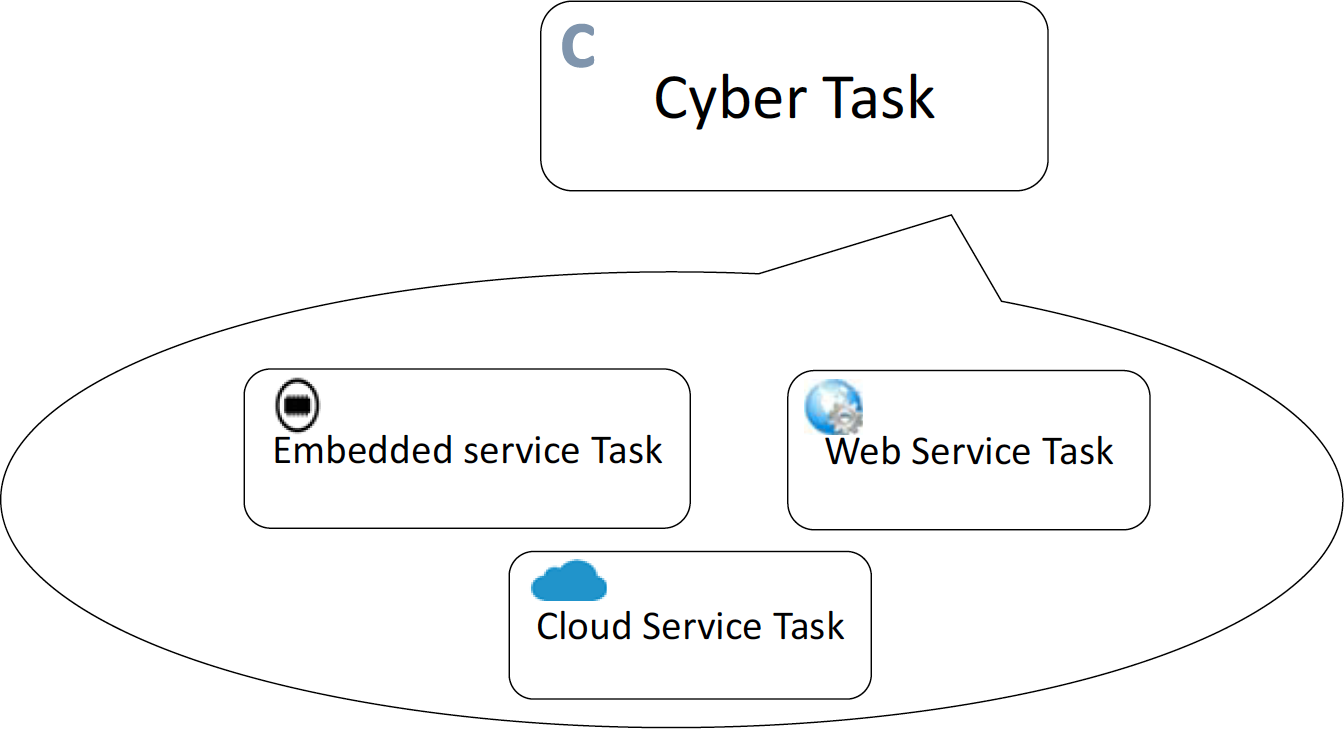
\includegraphics[height=4 cm,keepaspectratio,center]{figures/CyberTask}
	\caption{Physical Task\cite{BMPN4CPS}}
	\label{fig:cybertask}
\end{figure} 

In der Abbildung \ref{fig:bpmn4cpsProcess} ist ein minimaler Beispielprozess des \ac{bpmn4cps} zu sehen. Wie beschrieben sind die drei Standard Pools eines \ac{cps} zu sehen. Im physischen Prozess wird der gemessene Zustand einer pyhsischen Entität dem Controller mitgeteilt. Dieser leitet ihn an den Cyber Prozess weiter und führt selbst einen Embedded Service Task aus. Der Cyber Prozess führt zunächst einen Cloud Service Task aus und danach parallel einen Webservice Task sowie eine Cyber Activity, danach werden die Ergebnisse wieder dem Controller gesendet. Dieser wandelt sie in einen Befehl um welcher auf dem Physischen Prozess durch einen Actuator's activity ausgeführt wird, welche den Zustand einer physischen Entität ändert. 

\begin{figure}[H]
	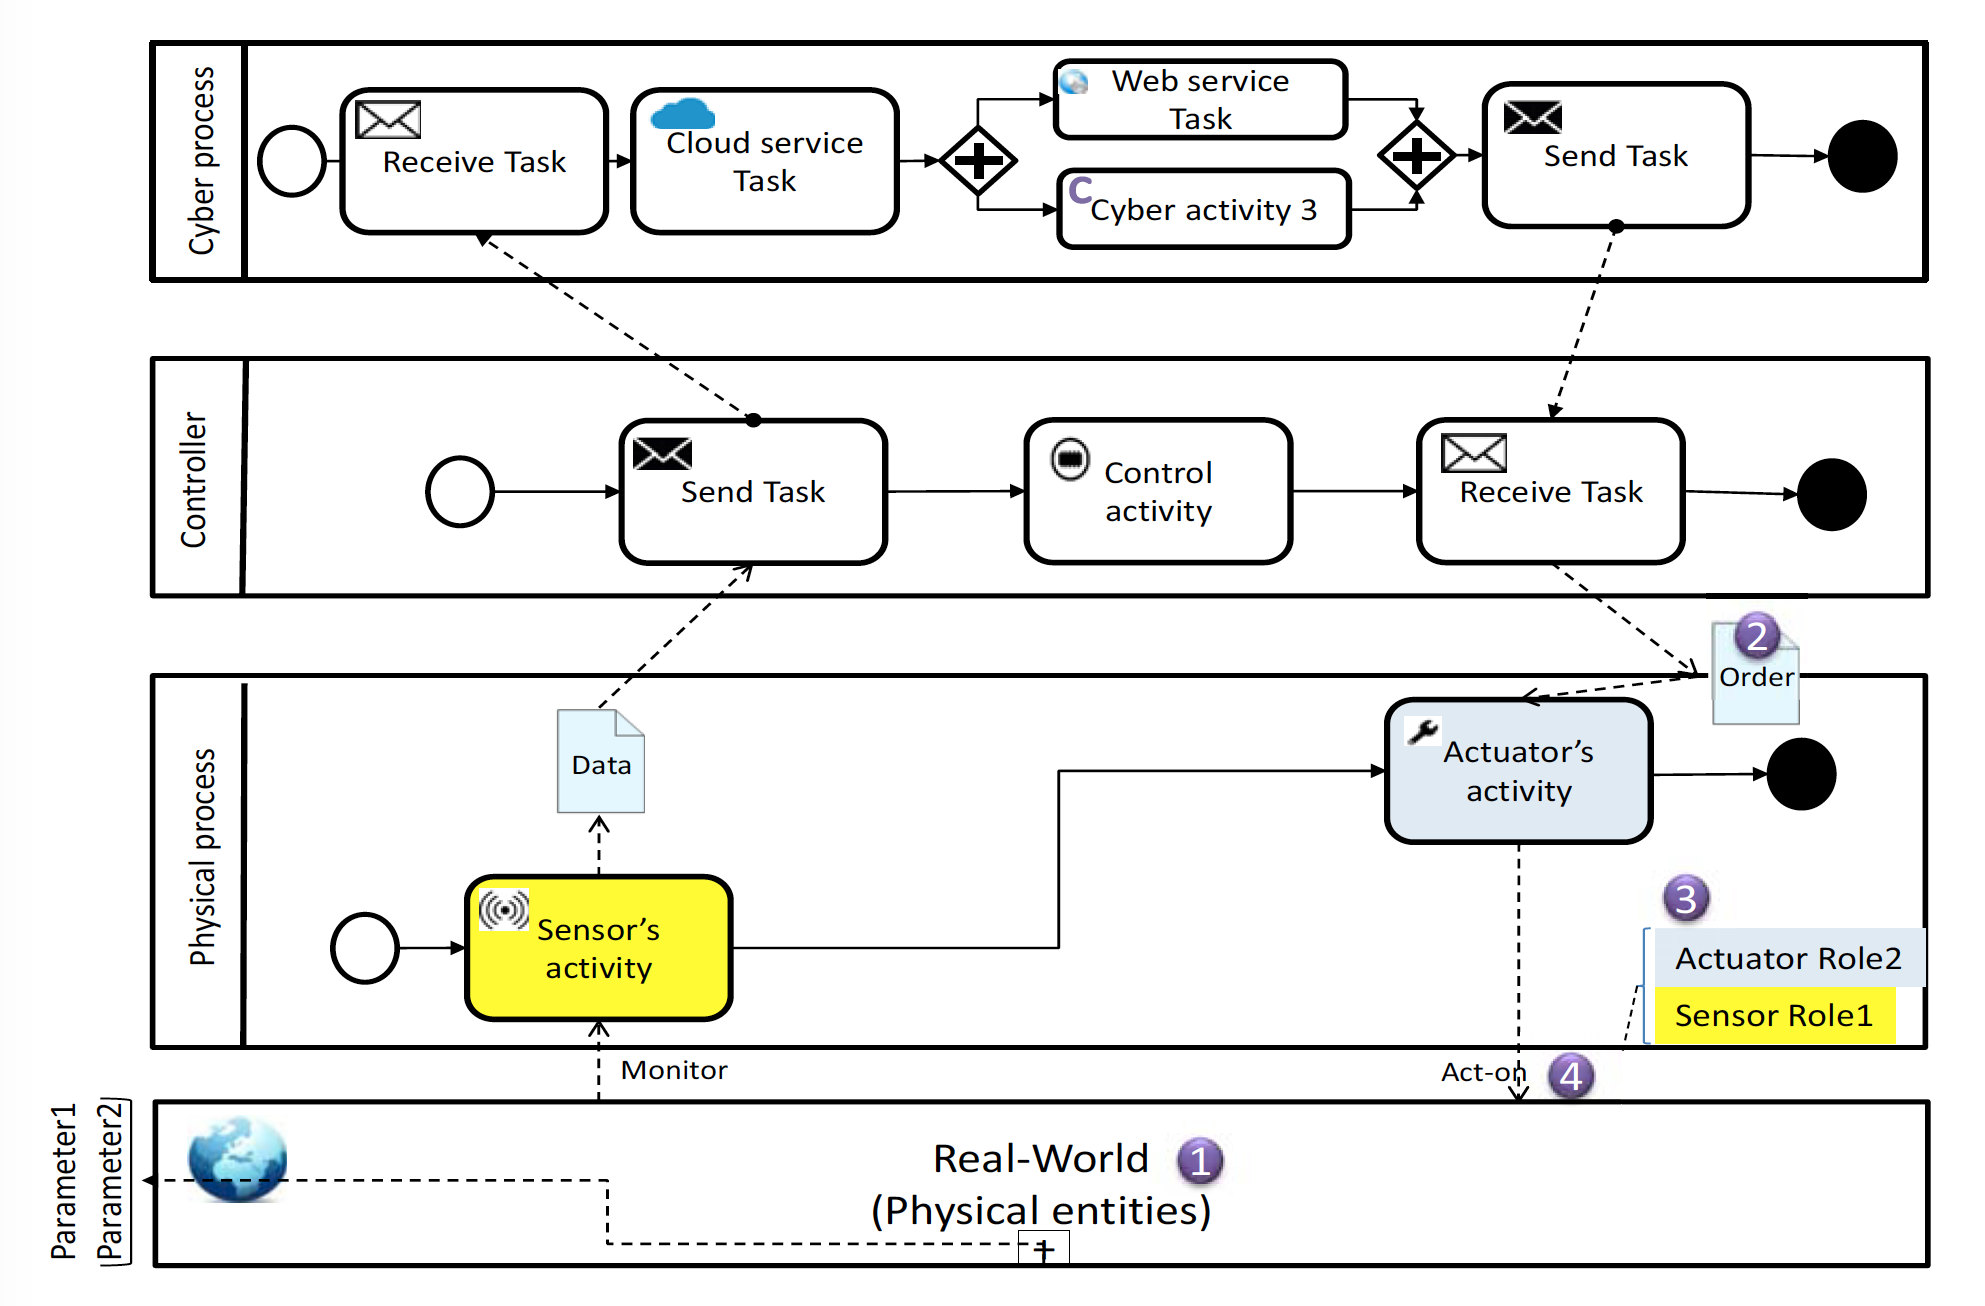
\includegraphics[height=11cm,keepaspectratio,center]{figures/bpmn4cpsProcess}
	\caption{Beispielprozess nach \ac{bpmn4cps} \cite{BMPN4CPS}}
	\label{fig:bpmn4cpsProcess}
\end{figure} 

Vorab: Strategie und Ziele des Unternehmens müssen klar sein
Modellerierung von IoT Workflows aus Ebene der Geschäftsarchitektur
Security ist für die Prozesse wichtig, muss aber in den darunterliegenden Schichten Anwendungsarhcitektur, Informationsarchiektur und Technologische Archiektur umgesetzt werden \cite{enterpricearichitecture}. Also von der Software die diese Prozesse ausführt. Das Modellierungskonzept muss also Möglichkeiten für die Umsetzung für Security bieten aber nicht selbst umsetzen.
%TODO https://www.bitkom.org/noindex/Publikationen/2011/Leitfaden/Leitfaden-EAM-Enterprise-Architecture-Management/EAM-Enterprise-Architecture-Management-BITKOM-Leitfaden.pdf

%Security kann anhand anhand von Pasrameter der Resourcen, Resourcen wählen die beispielsweise nur verschlüsslte Kommunikation akzeptieren. (IOTA)
%Security ist für die Prozesse wichtig, muss aber in den darunterliegenden Schichten Anwendungsarhcitektur, Informationsarchiektur und Technologische Archiektur umgesetzt werden. Also von der Software die diese Prozesse ausführt.

\subsection{Auswahl eines Modellierungskonzeptes}

\newpage

\section{Anwendung des Konzeptes}

use Cases: Max IoT Leasingrate, chris beispiel. Max Beispiel nur bedingt geeignet, da kein aktiver IoT bezug, zieht die Daten über die Nutzung der Gabelstapler aus Linde Connect System und nicht über IoT Device.
Eventuell besser Konzept belegen anhand von Chris Beispiel, Fahrstilbedingte Versicherungsraten. 

Fallbeispiel Chris: Fahrstilbedingter Versicherungstarif

- Bislang Kalkulation aufgrund von Statistischen Werten (Risikomerkmale) wie Regionalklasse, Typklasse. Diese Kalkulation fällt  schlechten Fahrern zugunsten aus und benachteiligt vorsichtige Fahrer.
- Durch Auswertung der von IoT Sensoren gesammelten Daten können per Complex Event Processing aus einer großen Menge einzelner Events Muster erkannt werden welche sich in Fahrstilen Zusammenfassen lassen.
- Einbezug des Fahrstils fördert vorsichtiges fahren und bietet Wettbewerbsvorteil gegenüber anderen Versicherungen.

\newpage

\subsection{Bewertung des Modellierungskonzeptes}

\section{Schlussteil}

\subsection{Ergebnis}

\subsection{Fazit}

Durch die erweiterte Darstellungsmöglichkeit des von dem \acl{iota} Projekt bereitgestellten \acl{iapmc} ist eine sinnvolle Darstellung von \ac{iot} Prozessen möglich und die erweiterten Metadaten ermöglichen eine einfache Umsetzung des Geschäftsprozesses. Diese Metadaten ermöglichen es mit den standardmäßig vorhanden Business Rules engines auf die den \ac{iot} Devices genierten Events einzugehen und den Prozessfluss somit zu automatisieren.\\
Bei der Modellierung der Prozesse müssen jedoch stets die Funktionalitäten der einzelnen \ac{iot} Devices berücksichtigt werden, da diese für den Informationsfluss sowie dessen Verarbeitung beachtet werden müssen. So sind die in \ref{fig:iotdevices} dargestellten "dumd Devices" lediglich in der Lage Daten zu sammeln und nicht auszuwerten, diese müssen also an einen weiteren Prozess Teilnehmer mitgeteilt werden welcher in der Lage ist die Auswertung der Daten und damit den weiteren Prozessablauf zu bestimmen übermittelt werden.\\

\subsection{Weiterführende Arbeit/ Ausblick}
Wie kommen wir zu automatisierbaren abläufen? -> Darstellung des Prozesses mit IoT-A und ausführung in BPMN Engine engies müssen IoT Spezifische Erweiterung akzeptieren\\
Workflow = automatisierte Ausführung von Business Processes

Problem, Nutzer müssen neue Technologie akzeptieren, Datenschutz esetze müssen eingehalten werden
\newpage

\addsec{Literaturverzeichnis}
\printbibliography[heading=none]
\newpage
\addsec{Anhang}
\subsection*{Unterbereich Anhang}
\end{document}
